\documentclass[conference]{IEEEtran}
\usepackage[protrusion=true,  expansion, tracking=true, spacing=true]{microtype} % typesetting

\usepackage{amsmath}
\usepackage{amsfonts}
\usepackage{graphicx}
\usepackage{booktabs} % \toprule <head>\\\midrule \cmidrule <bod>\\\bottomrule
\usepackage{csquotes}

\usepackage{siunitx}
\usepackage{epsfig}
\usepackage{subfigure}
\usepackage{calc}
\usepackage{amssymb}
\usepackage{amstext}
\usepackage{amsthm}
\usepackage{multicol}
\usepackage{multirow}
\usepackage{pslatex}
\usepackage{xspace}  % fixes spaces, as in \newcommand{\eg}{e.g.\xspace}
\usepackage{pgf}


\usepackage{cite}
\usepackage{amsmath,amssymb,amsfonts}
\usepackage{algorithmic}
\usepackage{graphicx}
\usepackage{textcomp}
\usepackage{xcolor}


% Abbreviations
\newcommand{\et}{et al.\xspace}
\newcommand{\eg}{e.g.\xspace}

\subfigtopskip=0pt
\subfigcapskip=0pt
\subfigbottomskip=0pt

\begin{document}

\title{Inferring Phone Location State}

\author{\IEEEauthorblockN{Steven Chen}
\IEEEauthorblockA{\textit{Electrical Engineering and Computer Science} \\
\textit{University of California, Berkeley}\\
Berkeley, United States \\
scchen@berkeley.edu}
\and
\IEEEauthorblockN{Won Park}
\IEEEauthorblockA{\textit{Electrical Engineering and Computer Science} \\
\textit{University of California, Berkeley}\\
Berkeley, United States \\
wonpark@berkeley.edu}
\and
\IEEEauthorblockN{Joanna Yang}
\IEEEauthorblockA{\textit{Electrical Engineering and Computer Science} \\
\textit{University of California, Berkeley}\\
Berkeley, United States \\
joannayangg@berkeley.edu}
\and
\IEEEauthorblockN{David Wagner}
\IEEEauthorblockA{\textit{Electrical Engineering and Computer Science} \\
\textit{University of California, Berkeley}\\
Berkeley, United States \\
daw@berkeley.edu}
}


\maketitle


\begin {abstract}Smartphone sensors are becoming more universal and more accurate. In this paper, we aim to distinguish between four common positions or states a phone can be in: in the hand, pocket, backpack, or on a table. Using a uniquely designed neural network and data from the accelerometer and the screen state, we achieve a 92\% accuracy on the same phone. We also explore extending this to different phones and propose an acceleration calibration technique to do so. 
\end{abstract}

\begin{IEEEkeywords}
Sensors, Smartphone, Position
\end{IEEEkeywords}

\section{Introduction}
With the recent proliferation of smartphones with sensors, such as light sensors and accelerometers,
 combined with the wide usage of smartphones over traditional phones, 
 there has been an explosion of applications utilizing sensors,
 including activity detection \cite{Martin2013} to user authentication \cite{Kumar17,Primo14}

Knowing, a priori, the position of the phone (e.g. in a bag, in a user's pocket, etc.), 
 which we will call \textit{phone state}, can prove to be useful.
For example, a phone's vibration intensity can be adjusted based on where the phone is positioned on the person, potentially prolonging battery usage \cite{Fujinami2013}.
In another example, CO2 and pollution sensors could be turned off automatically if the phone were deemed to be in a pocket or backpack \cite{Miluzzo2010} 

Not only that, but phone state can also be a powerful information tool that can enhance the quality of other classifiers.
For example, Mart\'{\i}n et al has shown that feeding phone state as an input to a classifier predicting activity will increase accuracy in certain instances \cite{Martin2013}.  
As another example, user authentication performance was augmented when a prior step was taken to infer phone state \cite{Primo14}.


In this paper, we discuss our methodology of automatically detecting and differentiating between four commonly identified phone states: table, backpack, hand, and table. 
To do this, we explore useful phone features that can be easily accessed from sensor data available to Android phone models, namely data from the accelerometer and the screen.
We then introduce a neural net architecture well-suited to process and learn from these features, 
and demonstrate that this architecture can achieve accuracy of 92\% in classifying a phone’s state provided data from a single phone model.
We then extend this to a different phone model and show that it could be possible to evaluate states on a 
 different phone, even if the phone has an accelerometer sensor that is calibrated differently.
To do this, we found that the acceleration values between the two phones can be adjusted with a simple offset.
When evaluating our twice classifier on the new phone, we achieve an accuracy of 78\% and 91\%.
Unfortunately, we were unable to investigate the root cause of this discrepancy further. 
While the work on this is preliminary, we belive it provides an important step toward the goal of a 
universal classifier that can detect different phone states across phone models. 


\section{Related work}
There has been much previous work involving smartphone sensors.
To note, this is a different set of work than the numerous pervious work that exist for wearable sensors \cite{Kunze2005,Atallah}.
We focus on smartphone sensors since we believe they are more readily accesible, prevalent, and versatile than wearable sensors.

Work by Khan et al, utilized accelerometer values to classify phone state 
but was limited to distinguishing between whether the phone was in the upper or lower half of the body \cite{Khan2010}.
Similarly, Miluzzo et al. proposed the use of various sensors to classify different phone locations, 
but only recognized two states: inside and outside of a pocket \cite{Miluzzo2010}.
In contrast, our work distinguishes between more states: hand, pocket, bag, and backpack. 

Several other works tried to classify and distinguish between more states (e.g. hand, bag, pocket, etc.), but only used data from the accelerometer resulting in accuracies between 74.6\% to 84\% \cite{Fujinami2013,Coksun15}. 
Our work improves on this accuracy by utilizing additional data from the phone screen.

Park et al achieved an accuracy of 94\% in distinguishing between hand, ear, pocket, and backpack, but required that the participant be walking \cite{Park2012}. 
In contrast, our work does not require that the phone user perform a specific task in order to distinguish between states.
Rather, we train and validate our model on phone data collected throughout the entire day, 
 including times when the phone may be still and not actually on the user. 

Other works improved accuracy by using several additional sensors \cite{Yang13}.
For example, Wiese et al explored the idea of adding sensors that utilize capacitive sensing,  multi-spectral properties, as well as light and proximity sensing \cite{Wiese2013}.
They were able to achieve accuracies of 85\% to 100\%.
Similarly, Mart\'{\i}n et al used sensors like light, proximity, and acceleration sensors
to obtain phone state accuracy of 92.94\% \cite{Martin2013}, but to cost in file size.
Our work achieves similar accuracy rates but with data from much fewer sensors.  

In this paper, we take this idea further and utilize data from only two data sources: the accelerometer and the phone screen. 
Data from both sources are readily available, do not require specific user permissions, and are less energy draining than previously studied sensors.
Furthermore, unlike previous work, we also train and validate our model on phone data collected throughout the entire day, and not just during specific tasks (e.g. walking).
This includes times when the phone may be still and not actually directly on the user.
An example of this may be if the phone is left on a table or in a backpack. 








\section{Approach}

\subsection{Problem}
We want to predict the state of an user's phone based on the sensor data collected on the phone. 
From our observations and prior research, the most common states of the phone would be in a user's: backpack, pocket, hand, or on a table.
Upon a cursory observation of accelerometer traces, these phone states also appeared to be distinguishable and motivated
our approach to use deep learning to classify these states.
Sample accelerometer traces for the states, measured on a Nexus 5X
smartphone are shown in Figure ~\ref{fig:AccelDiffStates}.

\begin{figure}[h]
\begin{center}
 \scalebox{0.1}{%% Creator: Matplotlib, PGF backend
%%
%% To include the figure in your LaTeX document, write
%%   \input{<filename>.pgf}
%%
%% Make sure the required packages are loaded in your preamble
%%   \usepackage{pgf}
%%
%% Figures using additional raster images can only be included by \input if
%% they are in the same directory as the main LaTeX file. For loading figures
%% from other directories you can use the `import` package
%%   \usepackage{import}
%% and then include the figures with
%%   \import{<path to file>}{<filename>.pgf}
%%
%% Matplotlib used the following preamble
%%   \usepackage{fontspec}
%%   \setmainfont{Times New Roman}
%%   \setsansfont{Lucida Grande}
%%   \setmonofont{Andale Mono}
%%
\begingroup%
\makeatletter%
\begin{pgfpicture}%
\pgfpathrectangle{\pgfpointorigin}{\pgfqpoint{7.500000in}{5.000000in}}%
\pgfusepath{use as bounding box, clip}%
\begin{pgfscope}%
\pgfsetbuttcap%
\pgfsetmiterjoin%
\definecolor{currentfill}{rgb}{1.000000,1.000000,1.000000}%
\pgfsetfillcolor{currentfill}%
\pgfsetlinewidth{0.000000pt}%
\definecolor{currentstroke}{rgb}{1.000000,1.000000,1.000000}%
\pgfsetstrokecolor{currentstroke}%
\pgfsetdash{}{0pt}%
\pgfpathmoveto{\pgfqpoint{0.000000in}{0.000000in}}%
\pgfpathlineto{\pgfqpoint{7.500000in}{0.000000in}}%
\pgfpathlineto{\pgfqpoint{7.500000in}{5.000000in}}%
\pgfpathlineto{\pgfqpoint{0.000000in}{5.000000in}}%
\pgfpathclose%
\pgfusepath{fill}%
\end{pgfscope}%
\begin{pgfscope}%
\pgfsetbuttcap%
\pgfsetmiterjoin%
\definecolor{currentfill}{rgb}{1.000000,1.000000,1.000000}%
\pgfsetfillcolor{currentfill}%
\pgfsetlinewidth{0.000000pt}%
\definecolor{currentstroke}{rgb}{0.000000,0.000000,0.000000}%
\pgfsetstrokecolor{currentstroke}%
\pgfsetstrokeopacity{0.000000}%
\pgfsetdash{}{0pt}%
\pgfpathmoveto{\pgfqpoint{0.646528in}{0.580556in}}%
\pgfpathlineto{\pgfqpoint{7.301389in}{0.580556in}}%
\pgfpathlineto{\pgfqpoint{7.301389in}{4.627778in}}%
\pgfpathlineto{\pgfqpoint{0.646528in}{4.627778in}}%
\pgfpathclose%
\pgfusepath{fill}%
\end{pgfscope}%
\begin{pgfscope}%
\pgfsetbuttcap%
\pgfsetroundjoin%
\definecolor{currentfill}{rgb}{0.000000,0.000000,0.000000}%
\pgfsetfillcolor{currentfill}%
\pgfsetlinewidth{0.803000pt}%
\definecolor{currentstroke}{rgb}{0.000000,0.000000,0.000000}%
\pgfsetstrokecolor{currentstroke}%
\pgfsetdash{}{0pt}%
\pgfsys@defobject{currentmarker}{\pgfqpoint{0.000000in}{-0.048611in}}{\pgfqpoint{0.000000in}{0.000000in}}{%
\pgfpathmoveto{\pgfqpoint{0.000000in}{0.000000in}}%
\pgfpathlineto{\pgfqpoint{0.000000in}{-0.048611in}}%
\pgfusepath{stroke,fill}%
}%
\begin{pgfscope}%
\pgfsys@transformshift{0.949021in}{0.580556in}%
\pgfsys@useobject{currentmarker}{}%
\end{pgfscope}%
\end{pgfscope}%
\begin{pgfscope}%
\pgftext[x=0.949021in,y=0.483333in,,top]{\sffamily\fontsize{10.000000}{12.000000}\selectfont 0}%
\end{pgfscope}%
\begin{pgfscope}%
\pgfsetbuttcap%
\pgfsetroundjoin%
\definecolor{currentfill}{rgb}{0.000000,0.000000,0.000000}%
\pgfsetfillcolor{currentfill}%
\pgfsetlinewidth{0.803000pt}%
\definecolor{currentstroke}{rgb}{0.000000,0.000000,0.000000}%
\pgfsetstrokecolor{currentstroke}%
\pgfsetdash{}{0pt}%
\pgfsys@defobject{currentmarker}{\pgfqpoint{0.000000in}{-0.048611in}}{\pgfqpoint{0.000000in}{0.000000in}}{%
\pgfpathmoveto{\pgfqpoint{0.000000in}{0.000000in}}%
\pgfpathlineto{\pgfqpoint{0.000000in}{-0.048611in}}%
\pgfusepath{stroke,fill}%
}%
\begin{pgfscope}%
\pgfsys@transformshift{2.183690in}{0.580556in}%
\pgfsys@useobject{currentmarker}{}%
\end{pgfscope}%
\end{pgfscope}%
\begin{pgfscope}%
\pgftext[x=2.183690in,y=0.483333in,,top]{\sffamily\fontsize{10.000000}{12.000000}\selectfont 100}%
\end{pgfscope}%
\begin{pgfscope}%
\pgfsetbuttcap%
\pgfsetroundjoin%
\definecolor{currentfill}{rgb}{0.000000,0.000000,0.000000}%
\pgfsetfillcolor{currentfill}%
\pgfsetlinewidth{0.803000pt}%
\definecolor{currentstroke}{rgb}{0.000000,0.000000,0.000000}%
\pgfsetstrokecolor{currentstroke}%
\pgfsetdash{}{0pt}%
\pgfsys@defobject{currentmarker}{\pgfqpoint{0.000000in}{-0.048611in}}{\pgfqpoint{0.000000in}{0.000000in}}{%
\pgfpathmoveto{\pgfqpoint{0.000000in}{0.000000in}}%
\pgfpathlineto{\pgfqpoint{0.000000in}{-0.048611in}}%
\pgfusepath{stroke,fill}%
}%
\begin{pgfscope}%
\pgfsys@transformshift{3.418358in}{0.580556in}%
\pgfsys@useobject{currentmarker}{}%
\end{pgfscope}%
\end{pgfscope}%
\begin{pgfscope}%
\pgftext[x=3.418358in,y=0.483333in,,top]{\sffamily\fontsize{10.000000}{12.000000}\selectfont 200}%
\end{pgfscope}%
\begin{pgfscope}%
\pgfsetbuttcap%
\pgfsetroundjoin%
\definecolor{currentfill}{rgb}{0.000000,0.000000,0.000000}%
\pgfsetfillcolor{currentfill}%
\pgfsetlinewidth{0.803000pt}%
\definecolor{currentstroke}{rgb}{0.000000,0.000000,0.000000}%
\pgfsetstrokecolor{currentstroke}%
\pgfsetdash{}{0pt}%
\pgfsys@defobject{currentmarker}{\pgfqpoint{0.000000in}{-0.048611in}}{\pgfqpoint{0.000000in}{0.000000in}}{%
\pgfpathmoveto{\pgfqpoint{0.000000in}{0.000000in}}%
\pgfpathlineto{\pgfqpoint{0.000000in}{-0.048611in}}%
\pgfusepath{stroke,fill}%
}%
\begin{pgfscope}%
\pgfsys@transformshift{4.653026in}{0.580556in}%
\pgfsys@useobject{currentmarker}{}%
\end{pgfscope}%
\end{pgfscope}%
\begin{pgfscope}%
\pgftext[x=4.653026in,y=0.483333in,,top]{\sffamily\fontsize{10.000000}{12.000000}\selectfont 300}%
\end{pgfscope}%
\begin{pgfscope}%
\pgfsetbuttcap%
\pgfsetroundjoin%
\definecolor{currentfill}{rgb}{0.000000,0.000000,0.000000}%
\pgfsetfillcolor{currentfill}%
\pgfsetlinewidth{0.803000pt}%
\definecolor{currentstroke}{rgb}{0.000000,0.000000,0.000000}%
\pgfsetstrokecolor{currentstroke}%
\pgfsetdash{}{0pt}%
\pgfsys@defobject{currentmarker}{\pgfqpoint{0.000000in}{-0.048611in}}{\pgfqpoint{0.000000in}{0.000000in}}{%
\pgfpathmoveto{\pgfqpoint{0.000000in}{0.000000in}}%
\pgfpathlineto{\pgfqpoint{0.000000in}{-0.048611in}}%
\pgfusepath{stroke,fill}%
}%
\begin{pgfscope}%
\pgfsys@transformshift{5.887694in}{0.580556in}%
\pgfsys@useobject{currentmarker}{}%
\end{pgfscope}%
\end{pgfscope}%
\begin{pgfscope}%
\pgftext[x=5.887694in,y=0.483333in,,top]{\sffamily\fontsize{10.000000}{12.000000}\selectfont 400}%
\end{pgfscope}%
\begin{pgfscope}%
\pgfsetbuttcap%
\pgfsetroundjoin%
\definecolor{currentfill}{rgb}{0.000000,0.000000,0.000000}%
\pgfsetfillcolor{currentfill}%
\pgfsetlinewidth{0.803000pt}%
\definecolor{currentstroke}{rgb}{0.000000,0.000000,0.000000}%
\pgfsetstrokecolor{currentstroke}%
\pgfsetdash{}{0pt}%
\pgfsys@defobject{currentmarker}{\pgfqpoint{0.000000in}{-0.048611in}}{\pgfqpoint{0.000000in}{0.000000in}}{%
\pgfpathmoveto{\pgfqpoint{0.000000in}{0.000000in}}%
\pgfpathlineto{\pgfqpoint{0.000000in}{-0.048611in}}%
\pgfusepath{stroke,fill}%
}%
\begin{pgfscope}%
\pgfsys@transformshift{7.122362in}{0.580556in}%
\pgfsys@useobject{currentmarker}{}%
\end{pgfscope}%
\end{pgfscope}%
\begin{pgfscope}%
\pgftext[x=7.122362in,y=0.483333in,,top]{\sffamily\fontsize{10.000000}{12.000000}\selectfont 500}%
\end{pgfscope}%
\begin{pgfscope}%
\pgftext[x=3.973958in,y=0.293907in,,top]{\sffamily\fontsize{10.000000}{12.000000}\selectfont Time (ms)}%
\end{pgfscope}%
\begin{pgfscope}%
\pgfsetbuttcap%
\pgfsetroundjoin%
\definecolor{currentfill}{rgb}{0.000000,0.000000,0.000000}%
\pgfsetfillcolor{currentfill}%
\pgfsetlinewidth{0.803000pt}%
\definecolor{currentstroke}{rgb}{0.000000,0.000000,0.000000}%
\pgfsetstrokecolor{currentstroke}%
\pgfsetdash{}{0pt}%
\pgfsys@defobject{currentmarker}{\pgfqpoint{-0.048611in}{0.000000in}}{\pgfqpoint{0.000000in}{0.000000in}}{%
\pgfpathmoveto{\pgfqpoint{0.000000in}{0.000000in}}%
\pgfpathlineto{\pgfqpoint{-0.048611in}{0.000000in}}%
\pgfusepath{stroke,fill}%
}%
\begin{pgfscope}%
\pgfsys@transformshift{0.646528in}{0.874264in}%
\pgfsys@useobject{currentmarker}{}%
\end{pgfscope}%
\end{pgfscope}%
\begin{pgfscope}%
\pgftext[x=0.351009in,y=0.820723in,left,base]{\sffamily\fontsize{10.000000}{12.000000}\selectfont −2}%
\end{pgfscope}%
\begin{pgfscope}%
\pgfsetbuttcap%
\pgfsetroundjoin%
\definecolor{currentfill}{rgb}{0.000000,0.000000,0.000000}%
\pgfsetfillcolor{currentfill}%
\pgfsetlinewidth{0.803000pt}%
\definecolor{currentstroke}{rgb}{0.000000,0.000000,0.000000}%
\pgfsetstrokecolor{currentstroke}%
\pgfsetdash{}{0pt}%
\pgfsys@defobject{currentmarker}{\pgfqpoint{-0.048611in}{0.000000in}}{\pgfqpoint{0.000000in}{0.000000in}}{%
\pgfpathmoveto{\pgfqpoint{0.000000in}{0.000000in}}%
\pgfpathlineto{\pgfqpoint{-0.048611in}{0.000000in}}%
\pgfusepath{stroke,fill}%
}%
\begin{pgfscope}%
\pgfsys@transformshift{0.646528in}{1.380768in}%
\pgfsys@useobject{currentmarker}{}%
\end{pgfscope}%
\end{pgfscope}%
\begin{pgfscope}%
\pgftext[x=0.461483in,y=1.327227in,left,base]{\sffamily\fontsize{10.000000}{12.000000}\selectfont 0}%
\end{pgfscope}%
\begin{pgfscope}%
\pgfsetbuttcap%
\pgfsetroundjoin%
\definecolor{currentfill}{rgb}{0.000000,0.000000,0.000000}%
\pgfsetfillcolor{currentfill}%
\pgfsetlinewidth{0.803000pt}%
\definecolor{currentstroke}{rgb}{0.000000,0.000000,0.000000}%
\pgfsetstrokecolor{currentstroke}%
\pgfsetdash{}{0pt}%
\pgfsys@defobject{currentmarker}{\pgfqpoint{-0.048611in}{0.000000in}}{\pgfqpoint{0.000000in}{0.000000in}}{%
\pgfpathmoveto{\pgfqpoint{0.000000in}{0.000000in}}%
\pgfpathlineto{\pgfqpoint{-0.048611in}{0.000000in}}%
\pgfusepath{stroke,fill}%
}%
\begin{pgfscope}%
\pgfsys@transformshift{0.646528in}{1.887272in}%
\pgfsys@useobject{currentmarker}{}%
\end{pgfscope}%
\end{pgfscope}%
\begin{pgfscope}%
\pgftext[x=0.461483in,y=1.833731in,left,base]{\sffamily\fontsize{10.000000}{12.000000}\selectfont 2}%
\end{pgfscope}%
\begin{pgfscope}%
\pgfsetbuttcap%
\pgfsetroundjoin%
\definecolor{currentfill}{rgb}{0.000000,0.000000,0.000000}%
\pgfsetfillcolor{currentfill}%
\pgfsetlinewidth{0.803000pt}%
\definecolor{currentstroke}{rgb}{0.000000,0.000000,0.000000}%
\pgfsetstrokecolor{currentstroke}%
\pgfsetdash{}{0pt}%
\pgfsys@defobject{currentmarker}{\pgfqpoint{-0.048611in}{0.000000in}}{\pgfqpoint{0.000000in}{0.000000in}}{%
\pgfpathmoveto{\pgfqpoint{0.000000in}{0.000000in}}%
\pgfpathlineto{\pgfqpoint{-0.048611in}{0.000000in}}%
\pgfusepath{stroke,fill}%
}%
\begin{pgfscope}%
\pgfsys@transformshift{0.646528in}{2.393776in}%
\pgfsys@useobject{currentmarker}{}%
\end{pgfscope}%
\end{pgfscope}%
\begin{pgfscope}%
\pgftext[x=0.461483in,y=2.340235in,left,base]{\sffamily\fontsize{10.000000}{12.000000}\selectfont 4}%
\end{pgfscope}%
\begin{pgfscope}%
\pgfsetbuttcap%
\pgfsetroundjoin%
\definecolor{currentfill}{rgb}{0.000000,0.000000,0.000000}%
\pgfsetfillcolor{currentfill}%
\pgfsetlinewidth{0.803000pt}%
\definecolor{currentstroke}{rgb}{0.000000,0.000000,0.000000}%
\pgfsetstrokecolor{currentstroke}%
\pgfsetdash{}{0pt}%
\pgfsys@defobject{currentmarker}{\pgfqpoint{-0.048611in}{0.000000in}}{\pgfqpoint{0.000000in}{0.000000in}}{%
\pgfpathmoveto{\pgfqpoint{0.000000in}{0.000000in}}%
\pgfpathlineto{\pgfqpoint{-0.048611in}{0.000000in}}%
\pgfusepath{stroke,fill}%
}%
\begin{pgfscope}%
\pgfsys@transformshift{0.646528in}{2.900280in}%
\pgfsys@useobject{currentmarker}{}%
\end{pgfscope}%
\end{pgfscope}%
\begin{pgfscope}%
\pgftext[x=0.461483in,y=2.846739in,left,base]{\sffamily\fontsize{10.000000}{12.000000}\selectfont 6}%
\end{pgfscope}%
\begin{pgfscope}%
\pgfsetbuttcap%
\pgfsetroundjoin%
\definecolor{currentfill}{rgb}{0.000000,0.000000,0.000000}%
\pgfsetfillcolor{currentfill}%
\pgfsetlinewidth{0.803000pt}%
\definecolor{currentstroke}{rgb}{0.000000,0.000000,0.000000}%
\pgfsetstrokecolor{currentstroke}%
\pgfsetdash{}{0pt}%
\pgfsys@defobject{currentmarker}{\pgfqpoint{-0.048611in}{0.000000in}}{\pgfqpoint{0.000000in}{0.000000in}}{%
\pgfpathmoveto{\pgfqpoint{0.000000in}{0.000000in}}%
\pgfpathlineto{\pgfqpoint{-0.048611in}{0.000000in}}%
\pgfusepath{stroke,fill}%
}%
\begin{pgfscope}%
\pgfsys@transformshift{0.646528in}{3.406784in}%
\pgfsys@useobject{currentmarker}{}%
\end{pgfscope}%
\end{pgfscope}%
\begin{pgfscope}%
\pgftext[x=0.461483in,y=3.353243in,left,base]{\sffamily\fontsize{10.000000}{12.000000}\selectfont 8}%
\end{pgfscope}%
\begin{pgfscope}%
\pgfsetbuttcap%
\pgfsetroundjoin%
\definecolor{currentfill}{rgb}{0.000000,0.000000,0.000000}%
\pgfsetfillcolor{currentfill}%
\pgfsetlinewidth{0.803000pt}%
\definecolor{currentstroke}{rgb}{0.000000,0.000000,0.000000}%
\pgfsetstrokecolor{currentstroke}%
\pgfsetdash{}{0pt}%
\pgfsys@defobject{currentmarker}{\pgfqpoint{-0.048611in}{0.000000in}}{\pgfqpoint{0.000000in}{0.000000in}}{%
\pgfpathmoveto{\pgfqpoint{0.000000in}{0.000000in}}%
\pgfpathlineto{\pgfqpoint{-0.048611in}{0.000000in}}%
\pgfusepath{stroke,fill}%
}%
\begin{pgfscope}%
\pgfsys@transformshift{0.646528in}{3.913288in}%
\pgfsys@useobject{currentmarker}{}%
\end{pgfscope}%
\end{pgfscope}%
\begin{pgfscope}%
\pgftext[x=0.373660in,y=3.859747in,left,base]{\sffamily\fontsize{10.000000}{12.000000}\selectfont 10}%
\end{pgfscope}%
\begin{pgfscope}%
\pgfsetbuttcap%
\pgfsetroundjoin%
\definecolor{currentfill}{rgb}{0.000000,0.000000,0.000000}%
\pgfsetfillcolor{currentfill}%
\pgfsetlinewidth{0.803000pt}%
\definecolor{currentstroke}{rgb}{0.000000,0.000000,0.000000}%
\pgfsetstrokecolor{currentstroke}%
\pgfsetdash{}{0pt}%
\pgfsys@defobject{currentmarker}{\pgfqpoint{-0.048611in}{0.000000in}}{\pgfqpoint{0.000000in}{0.000000in}}{%
\pgfpathmoveto{\pgfqpoint{0.000000in}{0.000000in}}%
\pgfpathlineto{\pgfqpoint{-0.048611in}{0.000000in}}%
\pgfusepath{stroke,fill}%
}%
\begin{pgfscope}%
\pgfsys@transformshift{0.646528in}{4.419792in}%
\pgfsys@useobject{currentmarker}{}%
\end{pgfscope}%
\end{pgfscope}%
\begin{pgfscope}%
\pgftext[x=0.373660in,y=4.366251in,left,base]{\sffamily\fontsize{10.000000}{12.000000}\selectfont 12}%
\end{pgfscope}%
\begin{pgfscope}%
\pgftext[x=0.295454in,y=2.604167in,,bottom,rotate=90.000000]{\sffamily\fontsize{10.000000}{12.000000}\selectfont Acceleration (g)}%
\end{pgfscope}%
\begin{pgfscope}%
\pgfpathrectangle{\pgfqpoint{0.646528in}{0.580556in}}{\pgfqpoint{6.654861in}{4.047222in}} %
\pgfusepath{clip}%
\pgfsetrectcap%
\pgfsetroundjoin%
\pgfsetlinewidth{1.505625pt}%
\definecolor{currentstroke}{rgb}{0.121569,0.466667,0.705882}%
\pgfsetstrokecolor{currentstroke}%
\pgfsetdash{}{0pt}%
\pgfpathmoveto{\pgfqpoint{0.949021in}{1.073857in}}%
\pgfpathlineto{\pgfqpoint{1.072488in}{1.156954in}}%
\pgfpathlineto{\pgfqpoint{1.195955in}{1.223067in}}%
\pgfpathlineto{\pgfqpoint{1.319422in}{1.259460in}}%
\pgfpathlineto{\pgfqpoint{1.442889in}{1.180609in}}%
\pgfpathlineto{\pgfqpoint{1.566356in}{1.110250in}}%
\pgfpathlineto{\pgfqpoint{1.689822in}{1.279476in}}%
\pgfpathlineto{\pgfqpoint{1.813289in}{1.257033in}}%
\pgfpathlineto{\pgfqpoint{1.936756in}{1.099939in}}%
\pgfpathlineto{\pgfqpoint{2.060223in}{1.032006in}}%
\pgfpathlineto{\pgfqpoint{2.183690in}{1.125414in}}%
\pgfpathlineto{\pgfqpoint{2.307156in}{1.202445in}}%
\pgfpathlineto{\pgfqpoint{2.430623in}{1.199412in}}%
\pgfpathlineto{\pgfqpoint{2.554090in}{1.220641in}}%
\pgfpathlineto{\pgfqpoint{2.677557in}{1.457799in}}%
\pgfpathlineto{\pgfqpoint{2.801024in}{1.844168in}}%
\pgfpathlineto{\pgfqpoint{2.924490in}{1.881167in}}%
\pgfpathlineto{\pgfqpoint{3.047957in}{1.756219in}}%
\pgfpathlineto{\pgfqpoint{3.171424in}{1.559092in}}%
\pgfpathlineto{\pgfqpoint{3.294891in}{1.542715in}}%
\pgfpathlineto{\pgfqpoint{3.418358in}{1.630664in}}%
\pgfpathlineto{\pgfqpoint{3.541824in}{1.613075in}}%
\pgfpathlineto{\pgfqpoint{3.665291in}{1.614894in}}%
\pgfpathlineto{\pgfqpoint{3.788758in}{1.643402in}}%
\pgfpathlineto{\pgfqpoint{3.912225in}{1.653106in}}%
\pgfpathlineto{\pgfqpoint{4.035692in}{1.679794in}}%
\pgfpathlineto{\pgfqpoint{4.159159in}{1.614288in}}%
\pgfpathlineto{\pgfqpoint{4.282625in}{1.496012in}}%
\pgfpathlineto{\pgfqpoint{4.406092in}{1.395932in}}%
\pgfpathlineto{\pgfqpoint{4.529559in}{1.393506in}}%
\pgfpathlineto{\pgfqpoint{4.653026in}{1.434751in}}%
\pgfpathlineto{\pgfqpoint{4.776493in}{1.428685in}}%
\pgfpathlineto{\pgfqpoint{4.899959in}{1.425653in}}%
\pgfpathlineto{\pgfqpoint{5.023426in}{1.455980in}}%
\pgfpathlineto{\pgfqpoint{5.146893in}{1.499651in}}%
\pgfpathlineto{\pgfqpoint{5.270360in}{1.560305in}}%
\pgfpathlineto{\pgfqpoint{5.393827in}{1.625205in}}%
\pgfpathlineto{\pgfqpoint{5.517293in}{1.658565in}}%
\pgfpathlineto{\pgfqpoint{5.640760in}{1.605796in}}%
\pgfpathlineto{\pgfqpoint{5.764227in}{1.471750in}}%
\pgfpathlineto{\pgfqpoint{5.887694in}{1.291606in}}%
\pgfpathlineto{\pgfqpoint{6.011161in}{1.041104in}}%
\pgfpathlineto{\pgfqpoint{6.134628in}{0.833666in}}%
\pgfpathlineto{\pgfqpoint{6.258094in}{0.764520in}}%
\pgfpathlineto{\pgfqpoint{6.381561in}{0.868846in}}%
\pgfpathlineto{\pgfqpoint{6.505028in}{1.055661in}}%
\pgfpathlineto{\pgfqpoint{6.628495in}{1.194560in}}%
\pgfpathlineto{\pgfqpoint{6.751962in}{1.266132in}}%
\pgfpathlineto{\pgfqpoint{6.875428in}{1.274623in}}%
\pgfpathlineto{\pgfqpoint{6.998895in}{1.224280in}}%
\pgfusepath{stroke}%
\end{pgfscope}%
\begin{pgfscope}%
\pgfpathrectangle{\pgfqpoint{0.646528in}{0.580556in}}{\pgfqpoint{6.654861in}{4.047222in}} %
\pgfusepath{clip}%
\pgfsetrectcap%
\pgfsetroundjoin%
\pgfsetlinewidth{1.505625pt}%
\definecolor{currentstroke}{rgb}{1.000000,0.498039,0.054902}%
\pgfsetstrokecolor{currentstroke}%
\pgfsetdash{}{0pt}%
\pgfpathmoveto{\pgfqpoint{0.949021in}{2.340320in}}%
\pgfpathlineto{\pgfqpoint{1.072488in}{2.360943in}}%
\pgfpathlineto{\pgfqpoint{1.195955in}{2.262683in}}%
\pgfpathlineto{\pgfqpoint{1.319422in}{2.194143in}}%
\pgfpathlineto{\pgfqpoint{1.442889in}{2.123784in}}%
\pgfpathlineto{\pgfqpoint{1.566356in}{2.083146in}}%
\pgfpathlineto{\pgfqpoint{1.689822in}{2.233569in}}%
\pgfpathlineto{\pgfqpoint{1.813289in}{2.313632in}}%
\pgfpathlineto{\pgfqpoint{1.936756in}{2.286338in}}%
\pgfpathlineto{\pgfqpoint{2.060223in}{2.304534in}}%
\pgfpathlineto{\pgfqpoint{2.183690in}{2.360336in}}%
\pgfpathlineto{\pgfqpoint{2.307156in}{2.331829in}}%
\pgfpathlineto{\pgfqpoint{2.430623in}{2.293010in}}%
\pgfpathlineto{\pgfqpoint{2.554090in}{2.266928in}}%
\pgfpathlineto{\pgfqpoint{2.677557in}{2.156537in}}%
\pgfpathlineto{\pgfqpoint{2.801024in}{2.146226in}}%
\pgfpathlineto{\pgfqpoint{2.924490in}{2.138948in}}%
\pgfpathlineto{\pgfqpoint{3.047957in}{2.167455in}}%
\pgfpathlineto{\pgfqpoint{3.171424in}{2.246306in}}%
\pgfpathlineto{\pgfqpoint{3.294891in}{2.302108in}}%
\pgfpathlineto{\pgfqpoint{3.418358in}{2.287551in}}%
\pgfpathlineto{\pgfqpoint{3.541824in}{2.288157in}}%
\pgfpathlineto{\pgfqpoint{3.665291in}{2.232355in}}%
\pgfpathlineto{\pgfqpoint{3.788758in}{2.197782in}}%
\pgfpathlineto{\pgfqpoint{3.912225in}{2.179586in}}%
\pgfpathlineto{\pgfqpoint{4.035692in}{2.149259in}}%
\pgfpathlineto{\pgfqpoint{4.159159in}{2.146833in}}%
\pgfpathlineto{\pgfqpoint{4.282625in}{2.177767in}}%
\pgfpathlineto{\pgfqpoint{4.406092in}{2.155931in}}%
\pgfpathlineto{\pgfqpoint{4.529559in}{2.066163in}}%
\pgfpathlineto{\pgfqpoint{4.653026in}{1.978214in}}%
\pgfpathlineto{\pgfqpoint{4.776493in}{1.949706in}}%
\pgfpathlineto{\pgfqpoint{4.899959in}{1.943034in}}%
\pgfpathlineto{\pgfqpoint{5.023426in}{1.925444in}}%
\pgfpathlineto{\pgfqpoint{5.146893in}{1.931510in}}%
\pgfpathlineto{\pgfqpoint{5.270360in}{1.930903in}}%
\pgfpathlineto{\pgfqpoint{5.393827in}{1.912100in}}%
\pgfpathlineto{\pgfqpoint{5.517293in}{1.923625in}}%
\pgfpathlineto{\pgfqpoint{5.640760in}{1.942428in}}%
\pgfpathlineto{\pgfqpoint{5.764227in}{1.964263in}}%
\pgfpathlineto{\pgfqpoint{5.887694in}{1.979427in}}%
\pgfpathlineto{\pgfqpoint{6.011161in}{1.979427in}}%
\pgfpathlineto{\pgfqpoint{6.134628in}{1.980640in}}%
\pgfpathlineto{\pgfqpoint{6.258094in}{1.980640in}}%
\pgfpathlineto{\pgfqpoint{6.381561in}{1.935756in}}%
\pgfpathlineto{\pgfqpoint{6.505028in}{1.875708in}}%
\pgfpathlineto{\pgfqpoint{6.628495in}{1.827791in}}%
\pgfpathlineto{\pgfqpoint{6.751962in}{1.827184in}}%
\pgfpathlineto{\pgfqpoint{6.875428in}{1.867216in}}%
\pgfpathlineto{\pgfqpoint{6.998895in}{1.892691in}}%
\pgfusepath{stroke}%
\end{pgfscope}%
\begin{pgfscope}%
\pgfpathrectangle{\pgfqpoint{0.646528in}{0.580556in}}{\pgfqpoint{6.654861in}{4.047222in}} %
\pgfusepath{clip}%
\pgfsetrectcap%
\pgfsetroundjoin%
\pgfsetlinewidth{1.505625pt}%
\definecolor{currentstroke}{rgb}{0.172549,0.627451,0.172549}%
\pgfsetstrokecolor{currentstroke}%
\pgfsetdash{}{0pt}%
\pgfpathmoveto{\pgfqpoint{0.949021in}{3.806336in}}%
\pgfpathlineto{\pgfqpoint{1.072488in}{3.862138in}}%
\pgfpathlineto{\pgfqpoint{1.195955in}{3.927644in}}%
\pgfpathlineto{\pgfqpoint{1.319422in}{3.997397in}}%
\pgfpathlineto{\pgfqpoint{1.442889in}{3.994364in}}%
\pgfpathlineto{\pgfqpoint{1.566356in}{3.888826in}}%
\pgfpathlineto{\pgfqpoint{1.689822in}{3.820893in}}%
\pgfpathlineto{\pgfqpoint{1.813289in}{3.843335in}}%
\pgfpathlineto{\pgfqpoint{1.936756in}{3.841515in}}%
\pgfpathlineto{\pgfqpoint{2.060223in}{3.753567in}}%
\pgfpathlineto{\pgfqpoint{2.183690in}{3.780861in}}%
\pgfpathlineto{\pgfqpoint{2.307156in}{3.922792in}}%
\pgfpathlineto{\pgfqpoint{2.430623in}{4.125984in}}%
\pgfpathlineto{\pgfqpoint{2.554090in}{4.019232in}}%
\pgfpathlineto{\pgfqpoint{2.677557in}{3.771763in}}%
\pgfpathlineto{\pgfqpoint{2.801024in}{3.683814in}}%
\pgfpathlineto{\pgfqpoint{2.924490in}{3.555833in}}%
\pgfpathlineto{\pgfqpoint{3.047957in}{3.466065in}}%
\pgfpathlineto{\pgfqpoint{3.171424in}{3.331412in}}%
\pgfpathlineto{\pgfqpoint{3.294891in}{3.244677in}}%
\pgfpathlineto{\pgfqpoint{3.418358in}{3.187661in}}%
\pgfpathlineto{\pgfqpoint{3.541824in}{3.270758in}}%
\pgfpathlineto{\pgfqpoint{3.665291in}{3.443016in}}%
\pgfpathlineto{\pgfqpoint{3.788758in}{3.553407in}}%
\pgfpathlineto{\pgfqpoint{3.912225in}{3.486081in}}%
\pgfpathlineto{\pgfqpoint{4.035692in}{3.426033in}}%
\pgfpathlineto{\pgfqpoint{4.159159in}{3.466671in}}%
\pgfpathlineto{\pgfqpoint{4.282625in}{3.599504in}}%
\pgfpathlineto{\pgfqpoint{4.406092in}{3.752960in}}%
\pgfpathlineto{\pgfqpoint{4.529559in}{3.944021in}}%
\pgfpathlineto{\pgfqpoint{4.653026in}{4.163590in}}%
\pgfpathlineto{\pgfqpoint{4.776493in}{4.273374in}}%
\pgfpathlineto{\pgfqpoint{4.899959in}{4.250932in}}%
\pgfpathlineto{\pgfqpoint{5.023426in}{4.156311in}}%
\pgfpathlineto{\pgfqpoint{5.146893in}{3.977988in}}%
\pgfpathlineto{\pgfqpoint{5.270360in}{3.785713in}}%
\pgfpathlineto{\pgfqpoint{5.393827in}{3.657126in}}%
\pgfpathlineto{\pgfqpoint{5.517293in}{3.569177in}}%
\pgfpathlineto{\pgfqpoint{5.640760in}{3.508523in}}%
\pgfpathlineto{\pgfqpoint{5.764227in}{3.511556in}}%
\pgfpathlineto{\pgfqpoint{5.887694in}{3.644995in}}%
\pgfpathlineto{\pgfqpoint{6.011161in}{3.877908in}}%
\pgfpathlineto{\pgfqpoint{6.134628in}{4.171475in}}%
\pgfpathlineto{\pgfqpoint{6.258094in}{4.414699in}}%
\pgfpathlineto{\pgfqpoint{6.381561in}{4.443813in}}%
\pgfpathlineto{\pgfqpoint{6.505028in}{4.330996in}}%
\pgfpathlineto{\pgfqpoint{6.628495in}{4.178147in}}%
\pgfpathlineto{\pgfqpoint{6.751962in}{4.019839in}}%
\pgfpathlineto{\pgfqpoint{6.875428in}{3.951300in}}%
\pgfpathlineto{\pgfqpoint{6.998895in}{3.987086in}}%
\pgfusepath{stroke}%
\end{pgfscope}%
\begin{pgfscope}%
\pgfsetrectcap%
\pgfsetmiterjoin%
\pgfsetlinewidth{0.803000pt}%
\definecolor{currentstroke}{rgb}{0.000000,0.000000,0.000000}%
\pgfsetstrokecolor{currentstroke}%
\pgfsetdash{}{0pt}%
\pgfpathmoveto{\pgfqpoint{0.646528in}{0.580556in}}%
\pgfpathlineto{\pgfqpoint{0.646528in}{4.627778in}}%
\pgfusepath{stroke}%
\end{pgfscope}%
\begin{pgfscope}%
\pgfsetrectcap%
\pgfsetmiterjoin%
\pgfsetlinewidth{0.803000pt}%
\definecolor{currentstroke}{rgb}{0.000000,0.000000,0.000000}%
\pgfsetstrokecolor{currentstroke}%
\pgfsetdash{}{0pt}%
\pgfpathmoveto{\pgfqpoint{7.301389in}{0.580556in}}%
\pgfpathlineto{\pgfqpoint{7.301389in}{4.627778in}}%
\pgfusepath{stroke}%
\end{pgfscope}%
\begin{pgfscope}%
\pgfsetrectcap%
\pgfsetmiterjoin%
\pgfsetlinewidth{0.803000pt}%
\definecolor{currentstroke}{rgb}{0.000000,0.000000,0.000000}%
\pgfsetstrokecolor{currentstroke}%
\pgfsetdash{}{0pt}%
\pgfpathmoveto{\pgfqpoint{0.646528in}{0.580556in}}%
\pgfpathlineto{\pgfqpoint{7.301389in}{0.580556in}}%
\pgfusepath{stroke}%
\end{pgfscope}%
\begin{pgfscope}%
\pgfsetrectcap%
\pgfsetmiterjoin%
\pgfsetlinewidth{0.803000pt}%
\definecolor{currentstroke}{rgb}{0.000000,0.000000,0.000000}%
\pgfsetstrokecolor{currentstroke}%
\pgfsetdash{}{0pt}%
\pgfpathmoveto{\pgfqpoint{0.646528in}{4.627778in}}%
\pgfpathlineto{\pgfqpoint{7.301389in}{4.627778in}}%
\pgfusepath{stroke}%
\end{pgfscope}%
\begin{pgfscope}%
\pgftext[x=3.973958in,y=4.711111in,,base]{\sffamily\fontsize{12.000000}{14.400000}\selectfont Accelerometer Data (Backpack)}%
\end{pgfscope}%
\begin{pgfscope}%
\pgfsetbuttcap%
\pgfsetmiterjoin%
\definecolor{currentfill}{rgb}{1.000000,1.000000,1.000000}%
\pgfsetfillcolor{currentfill}%
\pgfsetfillopacity{0.800000}%
\pgfsetlinewidth{1.003750pt}%
\definecolor{currentstroke}{rgb}{0.800000,0.800000,0.800000}%
\pgfsetstrokecolor{currentstroke}%
\pgfsetstrokeopacity{0.800000}%
\pgfsetdash{}{0pt}%
\pgfpathmoveto{\pgfqpoint{6.672781in}{2.278361in}}%
\pgfpathlineto{\pgfqpoint{7.204167in}{2.278361in}}%
\pgfpathquadraticcurveto{\pgfqpoint{7.231944in}{2.278361in}}{\pgfqpoint{7.231944in}{2.306139in}}%
\pgfpathlineto{\pgfqpoint{7.231944in}{2.902194in}}%
\pgfpathquadraticcurveto{\pgfqpoint{7.231944in}{2.929972in}}{\pgfqpoint{7.204167in}{2.929972in}}%
\pgfpathlineto{\pgfqpoint{6.672781in}{2.929972in}}%
\pgfpathquadraticcurveto{\pgfqpoint{6.645003in}{2.929972in}}{\pgfqpoint{6.645003in}{2.902194in}}%
\pgfpathlineto{\pgfqpoint{6.645003in}{2.306139in}}%
\pgfpathquadraticcurveto{\pgfqpoint{6.645003in}{2.278361in}}{\pgfqpoint{6.672781in}{2.278361in}}%
\pgfpathclose%
\pgfusepath{stroke,fill}%
\end{pgfscope}%
\begin{pgfscope}%
\pgfsetrectcap%
\pgfsetroundjoin%
\pgfsetlinewidth{1.505625pt}%
\definecolor{currentstroke}{rgb}{0.121569,0.466667,0.705882}%
\pgfsetstrokecolor{currentstroke}%
\pgfsetdash{}{0pt}%
\pgfpathmoveto{\pgfqpoint{6.700559in}{2.815945in}}%
\pgfpathlineto{\pgfqpoint{6.978337in}{2.815945in}}%
\pgfusepath{stroke}%
\end{pgfscope}%
\begin{pgfscope}%
\pgftext[x=7.089448in,y=2.767334in,left,base]{\sffamily\fontsize{10.000000}{12.000000}\selectfont X}%
\end{pgfscope}%
\begin{pgfscope}%
\pgfsetrectcap%
\pgfsetroundjoin%
\pgfsetlinewidth{1.505625pt}%
\definecolor{currentstroke}{rgb}{1.000000,0.498039,0.054902}%
\pgfsetstrokecolor{currentstroke}%
\pgfsetdash{}{0pt}%
\pgfpathmoveto{\pgfqpoint{6.700559in}{2.612630in}}%
\pgfpathlineto{\pgfqpoint{6.978337in}{2.612630in}}%
\pgfusepath{stroke}%
\end{pgfscope}%
\begin{pgfscope}%
\pgftext[x=7.089448in,y=2.564019in,left,base]{\sffamily\fontsize{10.000000}{12.000000}\selectfont Y}%
\end{pgfscope}%
\begin{pgfscope}%
\pgfsetrectcap%
\pgfsetroundjoin%
\pgfsetlinewidth{1.505625pt}%
\definecolor{currentstroke}{rgb}{0.172549,0.627451,0.172549}%
\pgfsetstrokecolor{currentstroke}%
\pgfsetdash{}{0pt}%
\pgfpathmoveto{\pgfqpoint{6.700559in}{2.409315in}}%
\pgfpathlineto{\pgfqpoint{6.978337in}{2.409315in}}%
\pgfusepath{stroke}%
\end{pgfscope}%
\begin{pgfscope}%
\pgftext[x=7.089448in,y=2.360704in,left,base]{\sffamily\fontsize{10.000000}{12.000000}\selectfont Z}%
\end{pgfscope}%
\end{pgfpicture}%
\makeatother%
\endgroup%
}
  \scalebox{0.1}{%% Creator: Matplotlib, PGF backend
%%
%% To include the figure in your LaTeX document, write
%%   \input{<filename>.pgf}
%%
%% Make sure the required packages are loaded in your preamble
%%   \usepackage{pgf}
%%
%% Figures using additional raster images can only be included by \input if
%% they are in the same directory as the main LaTeX file. For loading figures
%% from other directories you can use the `import` package
%%   \usepackage{import}
%% and then include the figures with
%%   \import{<path to file>}{<filename>.pgf}
%%
%% Matplotlib used the following preamble
%%   \usepackage{fontspec}
%%   \setmainfont{Times New Roman}
%%   \setsansfont{Lucida Grande}
%%   \setmonofont{Andale Mono}
%%
\begingroup%
\makeatletter%
\begin{pgfpicture}%
\pgfpathrectangle{\pgfpointorigin}{\pgfqpoint{7.500000in}{5.000000in}}%
\pgfusepath{use as bounding box, clip}%
\begin{pgfscope}%
\pgfsetbuttcap%
\pgfsetmiterjoin%
\definecolor{currentfill}{rgb}{1.000000,1.000000,1.000000}%
\pgfsetfillcolor{currentfill}%
\pgfsetlinewidth{0.000000pt}%
\definecolor{currentstroke}{rgb}{1.000000,1.000000,1.000000}%
\pgfsetstrokecolor{currentstroke}%
\pgfsetdash{}{0pt}%
\pgfpathmoveto{\pgfqpoint{0.000000in}{0.000000in}}%
\pgfpathlineto{\pgfqpoint{7.500000in}{0.000000in}}%
\pgfpathlineto{\pgfqpoint{7.500000in}{5.000000in}}%
\pgfpathlineto{\pgfqpoint{0.000000in}{5.000000in}}%
\pgfpathclose%
\pgfusepath{fill}%
\end{pgfscope}%
\begin{pgfscope}%
\pgfsetbuttcap%
\pgfsetmiterjoin%
\definecolor{currentfill}{rgb}{1.000000,1.000000,1.000000}%
\pgfsetfillcolor{currentfill}%
\pgfsetlinewidth{0.000000pt}%
\definecolor{currentstroke}{rgb}{0.000000,0.000000,0.000000}%
\pgfsetstrokecolor{currentstroke}%
\pgfsetstrokeopacity{0.000000}%
\pgfsetdash{}{0pt}%
\pgfpathmoveto{\pgfqpoint{0.735069in}{0.580556in}}%
\pgfpathlineto{\pgfqpoint{7.301389in}{0.580556in}}%
\pgfpathlineto{\pgfqpoint{7.301389in}{4.627778in}}%
\pgfpathlineto{\pgfqpoint{0.735069in}{4.627778in}}%
\pgfpathclose%
\pgfusepath{fill}%
\end{pgfscope}%
\begin{pgfscope}%
\pgfsetbuttcap%
\pgfsetroundjoin%
\definecolor{currentfill}{rgb}{0.000000,0.000000,0.000000}%
\pgfsetfillcolor{currentfill}%
\pgfsetlinewidth{0.803000pt}%
\definecolor{currentstroke}{rgb}{0.000000,0.000000,0.000000}%
\pgfsetstrokecolor{currentstroke}%
\pgfsetdash{}{0pt}%
\pgfsys@defobject{currentmarker}{\pgfqpoint{0.000000in}{-0.048611in}}{\pgfqpoint{0.000000in}{0.000000in}}{%
\pgfpathmoveto{\pgfqpoint{0.000000in}{0.000000in}}%
\pgfpathlineto{\pgfqpoint{0.000000in}{-0.048611in}}%
\pgfusepath{stroke,fill}%
}%
\begin{pgfscope}%
\pgfsys@transformshift{1.033539in}{0.580556in}%
\pgfsys@useobject{currentmarker}{}%
\end{pgfscope}%
\end{pgfscope}%
\begin{pgfscope}%
\pgftext[x=1.033539in,y=0.483333in,,top]{\sffamily\fontsize{10.000000}{12.000000}\selectfont 0}%
\end{pgfscope}%
\begin{pgfscope}%
\pgfsetbuttcap%
\pgfsetroundjoin%
\definecolor{currentfill}{rgb}{0.000000,0.000000,0.000000}%
\pgfsetfillcolor{currentfill}%
\pgfsetlinewidth{0.803000pt}%
\definecolor{currentstroke}{rgb}{0.000000,0.000000,0.000000}%
\pgfsetstrokecolor{currentstroke}%
\pgfsetdash{}{0pt}%
\pgfsys@defobject{currentmarker}{\pgfqpoint{0.000000in}{-0.048611in}}{\pgfqpoint{0.000000in}{0.000000in}}{%
\pgfpathmoveto{\pgfqpoint{0.000000in}{0.000000in}}%
\pgfpathlineto{\pgfqpoint{0.000000in}{-0.048611in}}%
\pgfusepath{stroke,fill}%
}%
\begin{pgfscope}%
\pgfsys@transformshift{2.251780in}{0.580556in}%
\pgfsys@useobject{currentmarker}{}%
\end{pgfscope}%
\end{pgfscope}%
\begin{pgfscope}%
\pgftext[x=2.251780in,y=0.483333in,,top]{\sffamily\fontsize{10.000000}{12.000000}\selectfont 100}%
\end{pgfscope}%
\begin{pgfscope}%
\pgfsetbuttcap%
\pgfsetroundjoin%
\definecolor{currentfill}{rgb}{0.000000,0.000000,0.000000}%
\pgfsetfillcolor{currentfill}%
\pgfsetlinewidth{0.803000pt}%
\definecolor{currentstroke}{rgb}{0.000000,0.000000,0.000000}%
\pgfsetstrokecolor{currentstroke}%
\pgfsetdash{}{0pt}%
\pgfsys@defobject{currentmarker}{\pgfqpoint{0.000000in}{-0.048611in}}{\pgfqpoint{0.000000in}{0.000000in}}{%
\pgfpathmoveto{\pgfqpoint{0.000000in}{0.000000in}}%
\pgfpathlineto{\pgfqpoint{0.000000in}{-0.048611in}}%
\pgfusepath{stroke,fill}%
}%
\begin{pgfscope}%
\pgfsys@transformshift{3.470021in}{0.580556in}%
\pgfsys@useobject{currentmarker}{}%
\end{pgfscope}%
\end{pgfscope}%
\begin{pgfscope}%
\pgftext[x=3.470021in,y=0.483333in,,top]{\sffamily\fontsize{10.000000}{12.000000}\selectfont 200}%
\end{pgfscope}%
\begin{pgfscope}%
\pgfsetbuttcap%
\pgfsetroundjoin%
\definecolor{currentfill}{rgb}{0.000000,0.000000,0.000000}%
\pgfsetfillcolor{currentfill}%
\pgfsetlinewidth{0.803000pt}%
\definecolor{currentstroke}{rgb}{0.000000,0.000000,0.000000}%
\pgfsetstrokecolor{currentstroke}%
\pgfsetdash{}{0pt}%
\pgfsys@defobject{currentmarker}{\pgfqpoint{0.000000in}{-0.048611in}}{\pgfqpoint{0.000000in}{0.000000in}}{%
\pgfpathmoveto{\pgfqpoint{0.000000in}{0.000000in}}%
\pgfpathlineto{\pgfqpoint{0.000000in}{-0.048611in}}%
\pgfusepath{stroke,fill}%
}%
\begin{pgfscope}%
\pgfsys@transformshift{4.688262in}{0.580556in}%
\pgfsys@useobject{currentmarker}{}%
\end{pgfscope}%
\end{pgfscope}%
\begin{pgfscope}%
\pgftext[x=4.688262in,y=0.483333in,,top]{\sffamily\fontsize{10.000000}{12.000000}\selectfont 300}%
\end{pgfscope}%
\begin{pgfscope}%
\pgfsetbuttcap%
\pgfsetroundjoin%
\definecolor{currentfill}{rgb}{0.000000,0.000000,0.000000}%
\pgfsetfillcolor{currentfill}%
\pgfsetlinewidth{0.803000pt}%
\definecolor{currentstroke}{rgb}{0.000000,0.000000,0.000000}%
\pgfsetstrokecolor{currentstroke}%
\pgfsetdash{}{0pt}%
\pgfsys@defobject{currentmarker}{\pgfqpoint{0.000000in}{-0.048611in}}{\pgfqpoint{0.000000in}{0.000000in}}{%
\pgfpathmoveto{\pgfqpoint{0.000000in}{0.000000in}}%
\pgfpathlineto{\pgfqpoint{0.000000in}{-0.048611in}}%
\pgfusepath{stroke,fill}%
}%
\begin{pgfscope}%
\pgfsys@transformshift{5.906503in}{0.580556in}%
\pgfsys@useobject{currentmarker}{}%
\end{pgfscope}%
\end{pgfscope}%
\begin{pgfscope}%
\pgftext[x=5.906503in,y=0.483333in,,top]{\sffamily\fontsize{10.000000}{12.000000}\selectfont 400}%
\end{pgfscope}%
\begin{pgfscope}%
\pgfsetbuttcap%
\pgfsetroundjoin%
\definecolor{currentfill}{rgb}{0.000000,0.000000,0.000000}%
\pgfsetfillcolor{currentfill}%
\pgfsetlinewidth{0.803000pt}%
\definecolor{currentstroke}{rgb}{0.000000,0.000000,0.000000}%
\pgfsetstrokecolor{currentstroke}%
\pgfsetdash{}{0pt}%
\pgfsys@defobject{currentmarker}{\pgfqpoint{0.000000in}{-0.048611in}}{\pgfqpoint{0.000000in}{0.000000in}}{%
\pgfpathmoveto{\pgfqpoint{0.000000in}{0.000000in}}%
\pgfpathlineto{\pgfqpoint{0.000000in}{-0.048611in}}%
\pgfusepath{stroke,fill}%
}%
\begin{pgfscope}%
\pgfsys@transformshift{7.124744in}{0.580556in}%
\pgfsys@useobject{currentmarker}{}%
\end{pgfscope}%
\end{pgfscope}%
\begin{pgfscope}%
\pgftext[x=7.124744in,y=0.483333in,,top]{\sffamily\fontsize{10.000000}{12.000000}\selectfont 500}%
\end{pgfscope}%
\begin{pgfscope}%
\pgftext[x=4.018229in,y=0.293907in,,top]{\sffamily\fontsize{10.000000}{12.000000}\selectfont Time (ms)}%
\end{pgfscope}%
\begin{pgfscope}%
\pgfsetbuttcap%
\pgfsetroundjoin%
\definecolor{currentfill}{rgb}{0.000000,0.000000,0.000000}%
\pgfsetfillcolor{currentfill}%
\pgfsetlinewidth{0.803000pt}%
\definecolor{currentstroke}{rgb}{0.000000,0.000000,0.000000}%
\pgfsetstrokecolor{currentstroke}%
\pgfsetdash{}{0pt}%
\pgfsys@defobject{currentmarker}{\pgfqpoint{-0.048611in}{0.000000in}}{\pgfqpoint{0.000000in}{0.000000in}}{%
\pgfpathmoveto{\pgfqpoint{0.000000in}{0.000000in}}%
\pgfpathlineto{\pgfqpoint{-0.048611in}{0.000000in}}%
\pgfusepath{stroke,fill}%
}%
\begin{pgfscope}%
\pgfsys@transformshift{0.735069in}{0.639320in}%
\pgfsys@useobject{currentmarker}{}%
\end{pgfscope}%
\end{pgfscope}%
\begin{pgfscope}%
\pgftext[x=0.351728in,y=0.585778in,left,base]{\sffamily\fontsize{10.000000}{12.000000}\selectfont −20}%
\end{pgfscope}%
\begin{pgfscope}%
\pgfsetbuttcap%
\pgfsetroundjoin%
\definecolor{currentfill}{rgb}{0.000000,0.000000,0.000000}%
\pgfsetfillcolor{currentfill}%
\pgfsetlinewidth{0.803000pt}%
\definecolor{currentstroke}{rgb}{0.000000,0.000000,0.000000}%
\pgfsetstrokecolor{currentstroke}%
\pgfsetdash{}{0pt}%
\pgfsys@defobject{currentmarker}{\pgfqpoint{-0.048611in}{0.000000in}}{\pgfqpoint{0.000000in}{0.000000in}}{%
\pgfpathmoveto{\pgfqpoint{0.000000in}{0.000000in}}%
\pgfpathlineto{\pgfqpoint{-0.048611in}{0.000000in}}%
\pgfusepath{stroke,fill}%
}%
\begin{pgfscope}%
\pgfsys@transformshift{0.735069in}{1.228454in}%
\pgfsys@useobject{currentmarker}{}%
\end{pgfscope}%
\end{pgfscope}%
\begin{pgfscope}%
\pgftext[x=0.351728in,y=1.174913in,left,base]{\sffamily\fontsize{10.000000}{12.000000}\selectfont −15}%
\end{pgfscope}%
\begin{pgfscope}%
\pgfsetbuttcap%
\pgfsetroundjoin%
\definecolor{currentfill}{rgb}{0.000000,0.000000,0.000000}%
\pgfsetfillcolor{currentfill}%
\pgfsetlinewidth{0.803000pt}%
\definecolor{currentstroke}{rgb}{0.000000,0.000000,0.000000}%
\pgfsetstrokecolor{currentstroke}%
\pgfsetdash{}{0pt}%
\pgfsys@defobject{currentmarker}{\pgfqpoint{-0.048611in}{0.000000in}}{\pgfqpoint{0.000000in}{0.000000in}}{%
\pgfpathmoveto{\pgfqpoint{0.000000in}{0.000000in}}%
\pgfpathlineto{\pgfqpoint{-0.048611in}{0.000000in}}%
\pgfusepath{stroke,fill}%
}%
\begin{pgfscope}%
\pgfsys@transformshift{0.735069in}{1.817588in}%
\pgfsys@useobject{currentmarker}{}%
\end{pgfscope}%
\end{pgfscope}%
\begin{pgfscope}%
\pgftext[x=0.351728in,y=1.764047in,left,base]{\sffamily\fontsize{10.000000}{12.000000}\selectfont −10}%
\end{pgfscope}%
\begin{pgfscope}%
\pgfsetbuttcap%
\pgfsetroundjoin%
\definecolor{currentfill}{rgb}{0.000000,0.000000,0.000000}%
\pgfsetfillcolor{currentfill}%
\pgfsetlinewidth{0.803000pt}%
\definecolor{currentstroke}{rgb}{0.000000,0.000000,0.000000}%
\pgfsetstrokecolor{currentstroke}%
\pgfsetdash{}{0pt}%
\pgfsys@defobject{currentmarker}{\pgfqpoint{-0.048611in}{0.000000in}}{\pgfqpoint{0.000000in}{0.000000in}}{%
\pgfpathmoveto{\pgfqpoint{0.000000in}{0.000000in}}%
\pgfpathlineto{\pgfqpoint{-0.048611in}{0.000000in}}%
\pgfusepath{stroke,fill}%
}%
\begin{pgfscope}%
\pgfsys@transformshift{0.735069in}{2.406723in}%
\pgfsys@useobject{currentmarker}{}%
\end{pgfscope}%
\end{pgfscope}%
\begin{pgfscope}%
\pgftext[x=0.439551in,y=2.353181in,left,base]{\sffamily\fontsize{10.000000}{12.000000}\selectfont −5}%
\end{pgfscope}%
\begin{pgfscope}%
\pgfsetbuttcap%
\pgfsetroundjoin%
\definecolor{currentfill}{rgb}{0.000000,0.000000,0.000000}%
\pgfsetfillcolor{currentfill}%
\pgfsetlinewidth{0.803000pt}%
\definecolor{currentstroke}{rgb}{0.000000,0.000000,0.000000}%
\pgfsetstrokecolor{currentstroke}%
\pgfsetdash{}{0pt}%
\pgfsys@defobject{currentmarker}{\pgfqpoint{-0.048611in}{0.000000in}}{\pgfqpoint{0.000000in}{0.000000in}}{%
\pgfpathmoveto{\pgfqpoint{0.000000in}{0.000000in}}%
\pgfpathlineto{\pgfqpoint{-0.048611in}{0.000000in}}%
\pgfusepath{stroke,fill}%
}%
\begin{pgfscope}%
\pgfsys@transformshift{0.735069in}{2.995857in}%
\pgfsys@useobject{currentmarker}{}%
\end{pgfscope}%
\end{pgfscope}%
\begin{pgfscope}%
\pgftext[x=0.550024in,y=2.942316in,left,base]{\sffamily\fontsize{10.000000}{12.000000}\selectfont 0}%
\end{pgfscope}%
\begin{pgfscope}%
\pgfsetbuttcap%
\pgfsetroundjoin%
\definecolor{currentfill}{rgb}{0.000000,0.000000,0.000000}%
\pgfsetfillcolor{currentfill}%
\pgfsetlinewidth{0.803000pt}%
\definecolor{currentstroke}{rgb}{0.000000,0.000000,0.000000}%
\pgfsetstrokecolor{currentstroke}%
\pgfsetdash{}{0pt}%
\pgfsys@defobject{currentmarker}{\pgfqpoint{-0.048611in}{0.000000in}}{\pgfqpoint{0.000000in}{0.000000in}}{%
\pgfpathmoveto{\pgfqpoint{0.000000in}{0.000000in}}%
\pgfpathlineto{\pgfqpoint{-0.048611in}{0.000000in}}%
\pgfusepath{stroke,fill}%
}%
\begin{pgfscope}%
\pgfsys@transformshift{0.735069in}{3.584991in}%
\pgfsys@useobject{currentmarker}{}%
\end{pgfscope}%
\end{pgfscope}%
\begin{pgfscope}%
\pgftext[x=0.550024in,y=3.531450in,left,base]{\sffamily\fontsize{10.000000}{12.000000}\selectfont 5}%
\end{pgfscope}%
\begin{pgfscope}%
\pgfsetbuttcap%
\pgfsetroundjoin%
\definecolor{currentfill}{rgb}{0.000000,0.000000,0.000000}%
\pgfsetfillcolor{currentfill}%
\pgfsetlinewidth{0.803000pt}%
\definecolor{currentstroke}{rgb}{0.000000,0.000000,0.000000}%
\pgfsetstrokecolor{currentstroke}%
\pgfsetdash{}{0pt}%
\pgfsys@defobject{currentmarker}{\pgfqpoint{-0.048611in}{0.000000in}}{\pgfqpoint{0.000000in}{0.000000in}}{%
\pgfpathmoveto{\pgfqpoint{0.000000in}{0.000000in}}%
\pgfpathlineto{\pgfqpoint{-0.048611in}{0.000000in}}%
\pgfusepath{stroke,fill}%
}%
\begin{pgfscope}%
\pgfsys@transformshift{0.735069in}{4.174126in}%
\pgfsys@useobject{currentmarker}{}%
\end{pgfscope}%
\end{pgfscope}%
\begin{pgfscope}%
\pgftext[x=0.462202in,y=4.120584in,left,base]{\sffamily\fontsize{10.000000}{12.000000}\selectfont 10}%
\end{pgfscope}%
\begin{pgfscope}%
\pgftext[x=0.296172in,y=2.604167in,,bottom,rotate=90.000000]{\sffamily\fontsize{10.000000}{12.000000}\selectfont Acceleration (g)}%
\end{pgfscope}%
\begin{pgfscope}%
\pgfpathrectangle{\pgfqpoint{0.735069in}{0.580556in}}{\pgfqpoint{6.566319in}{4.047222in}} %
\pgfusepath{clip}%
\pgfsetrectcap%
\pgfsetroundjoin%
\pgfsetlinewidth{1.505625pt}%
\definecolor{currentstroke}{rgb}{0.121569,0.466667,0.705882}%
\pgfsetstrokecolor{currentstroke}%
\pgfsetdash{}{0pt}%
\pgfpathmoveto{\pgfqpoint{1.033539in}{2.372482in}}%
\pgfpathlineto{\pgfqpoint{1.155363in}{2.265812in}}%
\pgfpathlineto{\pgfqpoint{1.277187in}{2.102419in}}%
\pgfpathlineto{\pgfqpoint{1.399011in}{1.999135in}}%
\pgfpathlineto{\pgfqpoint{1.520835in}{1.906574in}}%
\pgfpathlineto{\pgfqpoint{1.642659in}{1.850699in}}%
\pgfpathlineto{\pgfqpoint{1.764483in}{1.783818in}}%
\pgfpathlineto{\pgfqpoint{1.886307in}{1.613371in}}%
\pgfpathlineto{\pgfqpoint{2.008131in}{1.413575in}}%
\pgfpathlineto{\pgfqpoint{2.129955in}{1.253004in}}%
\pgfpathlineto{\pgfqpoint{2.251780in}{1.153953in}}%
\pgfpathlineto{\pgfqpoint{2.373604in}{1.060263in}}%
\pgfpathlineto{\pgfqpoint{2.495428in}{0.764520in}}%
\pgfpathlineto{\pgfqpoint{2.617252in}{0.810518in}}%
\pgfpathlineto{\pgfqpoint{2.739076in}{1.219987in}}%
\pgfpathlineto{\pgfqpoint{2.860900in}{1.171167in}}%
\pgfpathlineto{\pgfqpoint{2.982724in}{1.196565in}}%
\pgfpathlineto{\pgfqpoint{3.104548in}{1.371245in}}%
\pgfpathlineto{\pgfqpoint{3.226372in}{1.551005in}}%
\pgfpathlineto{\pgfqpoint{3.348197in}{1.610549in}}%
\pgfpathlineto{\pgfqpoint{3.470021in}{1.561446in}}%
\pgfpathlineto{\pgfqpoint{3.591845in}{1.535484in}}%
\pgfpathlineto{\pgfqpoint{3.713669in}{1.752494in}}%
\pgfpathlineto{\pgfqpoint{3.835493in}{1.884845in}}%
\pgfpathlineto{\pgfqpoint{3.957317in}{1.882305in}}%
\pgfpathlineto{\pgfqpoint{4.079141in}{1.882587in}}%
\pgfpathlineto{\pgfqpoint{4.200965in}{1.752776in}}%
\pgfpathlineto{\pgfqpoint{4.322789in}{1.452800in}}%
\pgfpathlineto{\pgfqpoint{4.444614in}{1.233533in}}%
\pgfpathlineto{\pgfqpoint{4.566438in}{1.231557in}}%
\pgfpathlineto{\pgfqpoint{4.688262in}{1.686460in}}%
\pgfpathlineto{\pgfqpoint{4.810086in}{2.236181in}}%
\pgfpathlineto{\pgfqpoint{4.931910in}{2.452344in}}%
\pgfpathlineto{\pgfqpoint{5.053734in}{2.540108in}}%
\pgfpathlineto{\pgfqpoint{5.175558in}{2.590339in}}%
\pgfpathlineto{\pgfqpoint{5.297382in}{2.584977in}}%
\pgfpathlineto{\pgfqpoint{5.419206in}{2.532206in}}%
\pgfpathlineto{\pgfqpoint{5.541031in}{2.480564in}}%
\pgfpathlineto{\pgfqpoint{5.662855in}{2.405217in}}%
\pgfpathlineto{\pgfqpoint{5.784679in}{2.337772in}}%
\pgfpathlineto{\pgfqpoint{5.906503in}{2.324791in}}%
\pgfpathlineto{\pgfqpoint{6.028327in}{2.298264in}}%
\pgfpathlineto{\pgfqpoint{6.150151in}{2.283872in}}%
\pgfpathlineto{\pgfqpoint{6.271975in}{2.341441in}}%
\pgfpathlineto{\pgfqpoint{6.393799in}{2.430897in}}%
\pgfpathlineto{\pgfqpoint{6.515623in}{2.479153in}}%
\pgfpathlineto{\pgfqpoint{6.637447in}{2.476331in}}%
\pgfpathlineto{\pgfqpoint{6.759272in}{2.460528in}}%
\pgfpathlineto{\pgfqpoint{6.881096in}{2.433719in}}%
\pgfpathlineto{\pgfqpoint{7.002920in}{2.394776in}}%
\pgfusepath{stroke}%
\end{pgfscope}%
\begin{pgfscope}%
\pgfpathrectangle{\pgfqpoint{0.735069in}{0.580556in}}{\pgfqpoint{6.566319in}{4.047222in}} %
\pgfusepath{clip}%
\pgfsetrectcap%
\pgfsetroundjoin%
\pgfsetlinewidth{1.505625pt}%
\definecolor{currentstroke}{rgb}{1.000000,0.498039,0.054902}%
\pgfsetstrokecolor{currentstroke}%
\pgfsetdash{}{0pt}%
\pgfpathmoveto{\pgfqpoint{1.033539in}{2.625896in}}%
\pgfpathlineto{\pgfqpoint{1.155363in}{2.636055in}}%
\pgfpathlineto{\pgfqpoint{1.277187in}{2.628436in}}%
\pgfpathlineto{\pgfqpoint{1.399011in}{2.619688in}}%
\pgfpathlineto{\pgfqpoint{1.520835in}{2.641981in}}%
\pgfpathlineto{\pgfqpoint{1.642659in}{2.666250in}}%
\pgfpathlineto{\pgfqpoint{1.764483in}{2.692495in}}%
\pgfpathlineto{\pgfqpoint{1.886307in}{2.745830in}}%
\pgfpathlineto{\pgfqpoint{2.008131in}{2.805656in}}%
\pgfpathlineto{\pgfqpoint{2.129955in}{2.866893in}}%
\pgfpathlineto{\pgfqpoint{2.251780in}{2.923614in}}%
\pgfpathlineto{\pgfqpoint{2.373604in}{3.024923in}}%
\pgfpathlineto{\pgfqpoint{2.495428in}{3.326028in}}%
\pgfpathlineto{\pgfqpoint{2.617252in}{3.385290in}}%
\pgfpathlineto{\pgfqpoint{2.739076in}{3.272975in}}%
\pgfpathlineto{\pgfqpoint{2.860900in}{3.441447in}}%
\pgfpathlineto{\pgfqpoint{2.982724in}{3.651684in}}%
\pgfpathlineto{\pgfqpoint{3.104548in}{3.726184in}}%
\pgfpathlineto{\pgfqpoint{3.226372in}{3.597502in}}%
\pgfpathlineto{\pgfqpoint{3.348197in}{3.381903in}}%
\pgfpathlineto{\pgfqpoint{3.470021in}{3.225284in}}%
\pgfpathlineto{\pgfqpoint{3.591845in}{3.223026in}}%
\pgfpathlineto{\pgfqpoint{3.713669in}{3.176463in}}%
\pgfpathlineto{\pgfqpoint{3.835493in}{3.037058in}}%
\pgfpathlineto{\pgfqpoint{3.957317in}{2.928130in}}%
\pgfpathlineto{\pgfqpoint{4.079141in}{2.811864in}}%
\pgfpathlineto{\pgfqpoint{4.200965in}{2.687979in}}%
\pgfpathlineto{\pgfqpoint{4.322789in}{2.572843in}}%
\pgfpathlineto{\pgfqpoint{4.444614in}{2.469841in}}%
\pgfpathlineto{\pgfqpoint{4.566438in}{2.321969in}}%
\pgfpathlineto{\pgfqpoint{4.688262in}{2.007036in}}%
\pgfpathlineto{\pgfqpoint{4.810086in}{1.650621in}}%
\pgfpathlineto{\pgfqpoint{4.931910in}{1.619861in}}%
\pgfpathlineto{\pgfqpoint{5.053734in}{1.851828in}}%
\pgfpathlineto{\pgfqpoint{5.175558in}{2.156601in}}%
\pgfpathlineto{\pgfqpoint{5.297382in}{2.429486in}}%
\pgfpathlineto{\pgfqpoint{5.419206in}{2.663146in}}%
\pgfpathlineto{\pgfqpoint{5.541031in}{2.785620in}}%
\pgfpathlineto{\pgfqpoint{5.662855in}{2.873948in}}%
\pgfpathlineto{\pgfqpoint{5.784679in}{2.933491in}}%
\pgfpathlineto{\pgfqpoint{5.906503in}{2.963686in}}%
\pgfpathlineto{\pgfqpoint{6.028327in}{2.977232in}}%
\pgfpathlineto{\pgfqpoint{6.150151in}{3.013918in}}%
\pgfpathlineto{\pgfqpoint{6.271975in}{3.050886in}}%
\pgfpathlineto{\pgfqpoint{6.393799in}{3.062456in}}%
\pgfpathlineto{\pgfqpoint{6.515623in}{3.054836in}}%
\pgfpathlineto{\pgfqpoint{6.637447in}{3.052014in}}%
\pgfpathlineto{\pgfqpoint{6.759272in}{3.029156in}}%
\pgfpathlineto{\pgfqpoint{6.881096in}{2.985980in}}%
\pgfpathlineto{\pgfqpoint{7.002920in}{2.883825in}}%
\pgfusepath{stroke}%
\end{pgfscope}%
\begin{pgfscope}%
\pgfpathrectangle{\pgfqpoint{0.735069in}{0.580556in}}{\pgfqpoint{6.566319in}{4.047222in}} %
\pgfusepath{clip}%
\pgfsetrectcap%
\pgfsetroundjoin%
\pgfsetlinewidth{1.505625pt}%
\definecolor{currentstroke}{rgb}{0.172549,0.627451,0.172549}%
\pgfsetstrokecolor{currentstroke}%
\pgfsetdash{}{0pt}%
\pgfpathmoveto{\pgfqpoint{1.033539in}{3.260276in}}%
\pgfpathlineto{\pgfqpoint{1.155363in}{3.402222in}}%
\pgfpathlineto{\pgfqpoint{1.277187in}{3.493371in}}%
\pgfpathlineto{\pgfqpoint{1.399011in}{3.523002in}}%
\pgfpathlineto{\pgfqpoint{1.520835in}{3.523567in}}%
\pgfpathlineto{\pgfqpoint{1.642659in}{3.522720in}}%
\pgfpathlineto{\pgfqpoint{1.764483in}{3.504659in}}%
\pgfpathlineto{\pgfqpoint{1.886307in}{3.473053in}}%
\pgfpathlineto{\pgfqpoint{2.008131in}{3.464587in}}%
\pgfpathlineto{\pgfqpoint{2.129955in}{3.462894in}}%
\pgfpathlineto{\pgfqpoint{2.251780in}{3.448220in}}%
\pgfpathlineto{\pgfqpoint{2.373604in}{3.156427in}}%
\pgfpathlineto{\pgfqpoint{2.495428in}{1.676583in}}%
\pgfpathlineto{\pgfqpoint{2.617252in}{1.197411in}}%
\pgfpathlineto{\pgfqpoint{2.739076in}{2.340876in}}%
\pgfpathlineto{\pgfqpoint{2.860900in}{2.478306in}}%
\pgfpathlineto{\pgfqpoint{2.982724in}{2.333257in}}%
\pgfpathlineto{\pgfqpoint{3.104548in}{2.487055in}}%
\pgfpathlineto{\pgfqpoint{3.226372in}{2.797190in}}%
\pgfpathlineto{\pgfqpoint{3.348197in}{2.943650in}}%
\pgfpathlineto{\pgfqpoint{3.470021in}{3.045524in}}%
\pgfpathlineto{\pgfqpoint{3.591845in}{3.211738in}}%
\pgfpathlineto{\pgfqpoint{3.713669in}{3.099141in}}%
\pgfpathlineto{\pgfqpoint{3.835493in}{3.029438in}}%
\pgfpathlineto{\pgfqpoint{3.957317in}{3.048346in}}%
\pgfpathlineto{\pgfqpoint{4.079141in}{3.098577in}}%
\pgfpathlineto{\pgfqpoint{4.200965in}{3.144575in}}%
\pgfpathlineto{\pgfqpoint{4.322789in}{3.247577in}}%
\pgfpathlineto{\pgfqpoint{4.444614in}{3.408430in}}%
\pgfpathlineto{\pgfqpoint{4.566438in}{3.830315in}}%
\pgfpathlineto{\pgfqpoint{4.688262in}{4.443813in}}%
\pgfpathlineto{\pgfqpoint{4.810086in}{4.432525in}}%
\pgfpathlineto{\pgfqpoint{4.931910in}{4.249097in}}%
\pgfpathlineto{\pgfqpoint{5.053734in}{4.052123in}}%
\pgfpathlineto{\pgfqpoint{5.175558in}{3.776416in}}%
\pgfpathlineto{\pgfqpoint{5.297382in}{3.574927in}}%
\pgfpathlineto{\pgfqpoint{5.419206in}{3.450477in}}%
\pgfpathlineto{\pgfqpoint{5.541031in}{3.343807in}}%
\pgfpathlineto{\pgfqpoint{5.662855in}{3.248988in}}%
\pgfpathlineto{\pgfqpoint{5.784679in}{3.171948in}}%
\pgfpathlineto{\pgfqpoint{5.906503in}{3.182390in}}%
\pgfpathlineto{\pgfqpoint{6.028327in}{3.194524in}}%
\pgfpathlineto{\pgfqpoint{6.150151in}{3.228106in}}%
\pgfpathlineto{\pgfqpoint{6.271975in}{3.230928in}}%
\pgfpathlineto{\pgfqpoint{6.393799in}{3.173077in}}%
\pgfpathlineto{\pgfqpoint{6.515623in}{3.112405in}}%
\pgfpathlineto{\pgfqpoint{6.637447in}{3.068664in}}%
\pgfpathlineto{\pgfqpoint{6.759272in}{3.045524in}}%
\pgfpathlineto{\pgfqpoint{6.881096in}{3.090111in}}%
\pgfpathlineto{\pgfqpoint{7.002920in}{3.221897in}}%
\pgfusepath{stroke}%
\end{pgfscope}%
\begin{pgfscope}%
\pgfsetrectcap%
\pgfsetmiterjoin%
\pgfsetlinewidth{0.803000pt}%
\definecolor{currentstroke}{rgb}{0.000000,0.000000,0.000000}%
\pgfsetstrokecolor{currentstroke}%
\pgfsetdash{}{0pt}%
\pgfpathmoveto{\pgfqpoint{0.735069in}{0.580556in}}%
\pgfpathlineto{\pgfqpoint{0.735069in}{4.627778in}}%
\pgfusepath{stroke}%
\end{pgfscope}%
\begin{pgfscope}%
\pgfsetrectcap%
\pgfsetmiterjoin%
\pgfsetlinewidth{0.803000pt}%
\definecolor{currentstroke}{rgb}{0.000000,0.000000,0.000000}%
\pgfsetstrokecolor{currentstroke}%
\pgfsetdash{}{0pt}%
\pgfpathmoveto{\pgfqpoint{7.301389in}{0.580556in}}%
\pgfpathlineto{\pgfqpoint{7.301389in}{4.627778in}}%
\pgfusepath{stroke}%
\end{pgfscope}%
\begin{pgfscope}%
\pgfsetrectcap%
\pgfsetmiterjoin%
\pgfsetlinewidth{0.803000pt}%
\definecolor{currentstroke}{rgb}{0.000000,0.000000,0.000000}%
\pgfsetstrokecolor{currentstroke}%
\pgfsetdash{}{0pt}%
\pgfpathmoveto{\pgfqpoint{0.735069in}{0.580556in}}%
\pgfpathlineto{\pgfqpoint{7.301389in}{0.580556in}}%
\pgfusepath{stroke}%
\end{pgfscope}%
\begin{pgfscope}%
\pgfsetrectcap%
\pgfsetmiterjoin%
\pgfsetlinewidth{0.803000pt}%
\definecolor{currentstroke}{rgb}{0.000000,0.000000,0.000000}%
\pgfsetstrokecolor{currentstroke}%
\pgfsetdash{}{0pt}%
\pgfpathmoveto{\pgfqpoint{0.735069in}{4.627778in}}%
\pgfpathlineto{\pgfqpoint{7.301389in}{4.627778in}}%
\pgfusepath{stroke}%
\end{pgfscope}%
\begin{pgfscope}%
\pgftext[x=4.018229in,y=4.711111in,,base]{\sffamily\fontsize{12.000000}{14.400000}\selectfont Accelerometer Data (Pocket)}%
\end{pgfscope}%
\begin{pgfscope}%
\pgfsetbuttcap%
\pgfsetmiterjoin%
\definecolor{currentfill}{rgb}{1.000000,1.000000,1.000000}%
\pgfsetfillcolor{currentfill}%
\pgfsetfillopacity{0.800000}%
\pgfsetlinewidth{1.003750pt}%
\definecolor{currentstroke}{rgb}{0.800000,0.800000,0.800000}%
\pgfsetstrokecolor{currentstroke}%
\pgfsetstrokeopacity{0.800000}%
\pgfsetdash{}{0pt}%
\pgfpathmoveto{\pgfqpoint{6.672781in}{3.906722in}}%
\pgfpathlineto{\pgfqpoint{7.204167in}{3.906722in}}%
\pgfpathquadraticcurveto{\pgfqpoint{7.231944in}{3.906722in}}{\pgfqpoint{7.231944in}{3.934500in}}%
\pgfpathlineto{\pgfqpoint{7.231944in}{4.530556in}}%
\pgfpathquadraticcurveto{\pgfqpoint{7.231944in}{4.558333in}}{\pgfqpoint{7.204167in}{4.558333in}}%
\pgfpathlineto{\pgfqpoint{6.672781in}{4.558333in}}%
\pgfpathquadraticcurveto{\pgfqpoint{6.645003in}{4.558333in}}{\pgfqpoint{6.645003in}{4.530556in}}%
\pgfpathlineto{\pgfqpoint{6.645003in}{3.934500in}}%
\pgfpathquadraticcurveto{\pgfqpoint{6.645003in}{3.906722in}}{\pgfqpoint{6.672781in}{3.906722in}}%
\pgfpathclose%
\pgfusepath{stroke,fill}%
\end{pgfscope}%
\begin{pgfscope}%
\pgfsetrectcap%
\pgfsetroundjoin%
\pgfsetlinewidth{1.505625pt}%
\definecolor{currentstroke}{rgb}{0.121569,0.466667,0.705882}%
\pgfsetstrokecolor{currentstroke}%
\pgfsetdash{}{0pt}%
\pgfpathmoveto{\pgfqpoint{6.700559in}{4.444306in}}%
\pgfpathlineto{\pgfqpoint{6.978337in}{4.444306in}}%
\pgfusepath{stroke}%
\end{pgfscope}%
\begin{pgfscope}%
\pgftext[x=7.089448in,y=4.395695in,left,base]{\sffamily\fontsize{10.000000}{12.000000}\selectfont X}%
\end{pgfscope}%
\begin{pgfscope}%
\pgfsetrectcap%
\pgfsetroundjoin%
\pgfsetlinewidth{1.505625pt}%
\definecolor{currentstroke}{rgb}{1.000000,0.498039,0.054902}%
\pgfsetstrokecolor{currentstroke}%
\pgfsetdash{}{0pt}%
\pgfpathmoveto{\pgfqpoint{6.700559in}{4.240991in}}%
\pgfpathlineto{\pgfqpoint{6.978337in}{4.240991in}}%
\pgfusepath{stroke}%
\end{pgfscope}%
\begin{pgfscope}%
\pgftext[x=7.089448in,y=4.192380in,left,base]{\sffamily\fontsize{10.000000}{12.000000}\selectfont Y}%
\end{pgfscope}%
\begin{pgfscope}%
\pgfsetrectcap%
\pgfsetroundjoin%
\pgfsetlinewidth{1.505625pt}%
\definecolor{currentstroke}{rgb}{0.172549,0.627451,0.172549}%
\pgfsetstrokecolor{currentstroke}%
\pgfsetdash{}{0pt}%
\pgfpathmoveto{\pgfqpoint{6.700559in}{4.037677in}}%
\pgfpathlineto{\pgfqpoint{6.978337in}{4.037677in}}%
\pgfusepath{stroke}%
\end{pgfscope}%
\begin{pgfscope}%
\pgftext[x=7.089448in,y=3.989066in,left,base]{\sffamily\fontsize{10.000000}{12.000000}\selectfont Z}%
\end{pgfscope}%
\end{pgfpicture}%
\makeatother%
\endgroup%
}
  \scalebox{0.1}{%% Creator: Matplotlib, PGF backend
%%
%% To include the figure in your LaTeX document, write
%%   \input{<filename>.pgf}
%%
%% Make sure the required packages are loaded in your preamble
%%   \usepackage{pgf}
%%
%% Figures using additional raster images can only be included by \input if
%% they are in the same directory as the main LaTeX file. For loading figures
%% from other directories you can use the `import` package
%%   \usepackage{import}
%% and then include the figures with
%%   \import{<path to file>}{<filename>.pgf}
%%
%% Matplotlib used the following preamble
%%   \usepackage{fontspec}
%%   \setmainfont{Times New Roman}
%%   \setsansfont{Lucida Grande}
%%   \setmonofont{Andale Mono}
%%
\begingroup%
\makeatletter%
\begin{pgfpicture}%
\pgfpathrectangle{\pgfpointorigin}{\pgfqpoint{7.500000in}{5.000000in}}%
\pgfusepath{use as bounding box, clip}%
\begin{pgfscope}%
\pgfsetbuttcap%
\pgfsetmiterjoin%
\definecolor{currentfill}{rgb}{1.000000,1.000000,1.000000}%
\pgfsetfillcolor{currentfill}%
\pgfsetlinewidth{0.000000pt}%
\definecolor{currentstroke}{rgb}{1.000000,1.000000,1.000000}%
\pgfsetstrokecolor{currentstroke}%
\pgfsetdash{}{0pt}%
\pgfpathmoveto{\pgfqpoint{0.000000in}{0.000000in}}%
\pgfpathlineto{\pgfqpoint{7.500000in}{0.000000in}}%
\pgfpathlineto{\pgfqpoint{7.500000in}{5.000000in}}%
\pgfpathlineto{\pgfqpoint{0.000000in}{5.000000in}}%
\pgfpathclose%
\pgfusepath{fill}%
\end{pgfscope}%
\begin{pgfscope}%
\pgfsetbuttcap%
\pgfsetmiterjoin%
\definecolor{currentfill}{rgb}{1.000000,1.000000,1.000000}%
\pgfsetfillcolor{currentfill}%
\pgfsetlinewidth{0.000000pt}%
\definecolor{currentstroke}{rgb}{0.000000,0.000000,0.000000}%
\pgfsetstrokecolor{currentstroke}%
\pgfsetstrokeopacity{0.000000}%
\pgfsetdash{}{0pt}%
\pgfpathmoveto{\pgfqpoint{0.927500in}{0.809444in}}%
\pgfpathlineto{\pgfqpoint{7.205428in}{0.809444in}}%
\pgfpathlineto{\pgfqpoint{7.205428in}{4.468333in}}%
\pgfpathlineto{\pgfqpoint{0.927500in}{4.468333in}}%
\pgfpathclose%
\pgfusepath{fill}%
\end{pgfscope}%
\begin{pgfscope}%
\pgfsetbuttcap%
\pgfsetroundjoin%
\definecolor{currentfill}{rgb}{0.000000,0.000000,0.000000}%
\pgfsetfillcolor{currentfill}%
\pgfsetlinewidth{0.803000pt}%
\definecolor{currentstroke}{rgb}{0.000000,0.000000,0.000000}%
\pgfsetstrokecolor{currentstroke}%
\pgfsetdash{}{0pt}%
\pgfsys@defobject{currentmarker}{\pgfqpoint{0.000000in}{-0.048611in}}{\pgfqpoint{0.000000in}{0.000000in}}{%
\pgfpathmoveto{\pgfqpoint{0.000000in}{0.000000in}}%
\pgfpathlineto{\pgfqpoint{0.000000in}{-0.048611in}}%
\pgfusepath{stroke,fill}%
}%
\begin{pgfscope}%
\pgfsys@transformshift{1.212860in}{0.809444in}%
\pgfsys@useobject{currentmarker}{}%
\end{pgfscope}%
\end{pgfscope}%
\begin{pgfscope}%
\pgftext[x=1.212860in,y=0.712222in,,top]{\sffamily\fontsize{16.000000}{19.200000}\selectfont 0}%
\end{pgfscope}%
\begin{pgfscope}%
\pgfsetbuttcap%
\pgfsetroundjoin%
\definecolor{currentfill}{rgb}{0.000000,0.000000,0.000000}%
\pgfsetfillcolor{currentfill}%
\pgfsetlinewidth{0.803000pt}%
\definecolor{currentstroke}{rgb}{0.000000,0.000000,0.000000}%
\pgfsetstrokecolor{currentstroke}%
\pgfsetdash{}{0pt}%
\pgfsys@defobject{currentmarker}{\pgfqpoint{0.000000in}{-0.048611in}}{\pgfqpoint{0.000000in}{0.000000in}}{%
\pgfpathmoveto{\pgfqpoint{0.000000in}{0.000000in}}%
\pgfpathlineto{\pgfqpoint{0.000000in}{-0.048611in}}%
\pgfusepath{stroke,fill}%
}%
\begin{pgfscope}%
\pgfsys@transformshift{2.377597in}{0.809444in}%
\pgfsys@useobject{currentmarker}{}%
\end{pgfscope}%
\end{pgfscope}%
\begin{pgfscope}%
\pgftext[x=2.377597in,y=0.712222in,,top]{\sffamily\fontsize{16.000000}{19.200000}\selectfont 100}%
\end{pgfscope}%
\begin{pgfscope}%
\pgfsetbuttcap%
\pgfsetroundjoin%
\definecolor{currentfill}{rgb}{0.000000,0.000000,0.000000}%
\pgfsetfillcolor{currentfill}%
\pgfsetlinewidth{0.803000pt}%
\definecolor{currentstroke}{rgb}{0.000000,0.000000,0.000000}%
\pgfsetstrokecolor{currentstroke}%
\pgfsetdash{}{0pt}%
\pgfsys@defobject{currentmarker}{\pgfqpoint{0.000000in}{-0.048611in}}{\pgfqpoint{0.000000in}{0.000000in}}{%
\pgfpathmoveto{\pgfqpoint{0.000000in}{0.000000in}}%
\pgfpathlineto{\pgfqpoint{0.000000in}{-0.048611in}}%
\pgfusepath{stroke,fill}%
}%
\begin{pgfscope}%
\pgfsys@transformshift{3.542333in}{0.809444in}%
\pgfsys@useobject{currentmarker}{}%
\end{pgfscope}%
\end{pgfscope}%
\begin{pgfscope}%
\pgftext[x=3.542333in,y=0.712222in,,top]{\sffamily\fontsize{16.000000}{19.200000}\selectfont 200}%
\end{pgfscope}%
\begin{pgfscope}%
\pgfsetbuttcap%
\pgfsetroundjoin%
\definecolor{currentfill}{rgb}{0.000000,0.000000,0.000000}%
\pgfsetfillcolor{currentfill}%
\pgfsetlinewidth{0.803000pt}%
\definecolor{currentstroke}{rgb}{0.000000,0.000000,0.000000}%
\pgfsetstrokecolor{currentstroke}%
\pgfsetdash{}{0pt}%
\pgfsys@defobject{currentmarker}{\pgfqpoint{0.000000in}{-0.048611in}}{\pgfqpoint{0.000000in}{0.000000in}}{%
\pgfpathmoveto{\pgfqpoint{0.000000in}{0.000000in}}%
\pgfpathlineto{\pgfqpoint{0.000000in}{-0.048611in}}%
\pgfusepath{stroke,fill}%
}%
\begin{pgfscope}%
\pgfsys@transformshift{4.707069in}{0.809444in}%
\pgfsys@useobject{currentmarker}{}%
\end{pgfscope}%
\end{pgfscope}%
\begin{pgfscope}%
\pgftext[x=4.707069in,y=0.712222in,,top]{\sffamily\fontsize{16.000000}{19.200000}\selectfont 300}%
\end{pgfscope}%
\begin{pgfscope}%
\pgfsetbuttcap%
\pgfsetroundjoin%
\definecolor{currentfill}{rgb}{0.000000,0.000000,0.000000}%
\pgfsetfillcolor{currentfill}%
\pgfsetlinewidth{0.803000pt}%
\definecolor{currentstroke}{rgb}{0.000000,0.000000,0.000000}%
\pgfsetstrokecolor{currentstroke}%
\pgfsetdash{}{0pt}%
\pgfsys@defobject{currentmarker}{\pgfqpoint{0.000000in}{-0.048611in}}{\pgfqpoint{0.000000in}{0.000000in}}{%
\pgfpathmoveto{\pgfqpoint{0.000000in}{0.000000in}}%
\pgfpathlineto{\pgfqpoint{0.000000in}{-0.048611in}}%
\pgfusepath{stroke,fill}%
}%
\begin{pgfscope}%
\pgfsys@transformshift{5.871805in}{0.809444in}%
\pgfsys@useobject{currentmarker}{}%
\end{pgfscope}%
\end{pgfscope}%
\begin{pgfscope}%
\pgftext[x=5.871805in,y=0.712222in,,top]{\sffamily\fontsize{16.000000}{19.200000}\selectfont 400}%
\end{pgfscope}%
\begin{pgfscope}%
\pgfsetbuttcap%
\pgfsetroundjoin%
\definecolor{currentfill}{rgb}{0.000000,0.000000,0.000000}%
\pgfsetfillcolor{currentfill}%
\pgfsetlinewidth{0.803000pt}%
\definecolor{currentstroke}{rgb}{0.000000,0.000000,0.000000}%
\pgfsetstrokecolor{currentstroke}%
\pgfsetdash{}{0pt}%
\pgfsys@defobject{currentmarker}{\pgfqpoint{0.000000in}{-0.048611in}}{\pgfqpoint{0.000000in}{0.000000in}}{%
\pgfpathmoveto{\pgfqpoint{0.000000in}{0.000000in}}%
\pgfpathlineto{\pgfqpoint{0.000000in}{-0.048611in}}%
\pgfusepath{stroke,fill}%
}%
\begin{pgfscope}%
\pgfsys@transformshift{7.036542in}{0.809444in}%
\pgfsys@useobject{currentmarker}{}%
\end{pgfscope}%
\end{pgfscope}%
\begin{pgfscope}%
\pgftext[x=7.036542in,y=0.712222in,,top]{\sffamily\fontsize{16.000000}{19.200000}\selectfont 500}%
\end{pgfscope}%
\begin{pgfscope}%
\pgftext[x=4.066464in,y=0.442474in,,top]{\sffamily\fontsize{16.000000}{19.200000}\selectfont Time (ms)}%
\end{pgfscope}%
\begin{pgfscope}%
\pgfsetbuttcap%
\pgfsetroundjoin%
\definecolor{currentfill}{rgb}{0.000000,0.000000,0.000000}%
\pgfsetfillcolor{currentfill}%
\pgfsetlinewidth{0.803000pt}%
\definecolor{currentstroke}{rgb}{0.000000,0.000000,0.000000}%
\pgfsetstrokecolor{currentstroke}%
\pgfsetdash{}{0pt}%
\pgfsys@defobject{currentmarker}{\pgfqpoint{-0.048611in}{0.000000in}}{\pgfqpoint{0.000000in}{0.000000in}}{%
\pgfpathmoveto{\pgfqpoint{0.000000in}{0.000000in}}%
\pgfpathlineto{\pgfqpoint{-0.048611in}{0.000000in}}%
\pgfusepath{stroke,fill}%
}%
\begin{pgfscope}%
\pgfsys@transformshift{0.927500in}{0.813021in}%
\pgfsys@useobject{currentmarker}{}%
\end{pgfscope}%
\end{pgfscope}%
\begin{pgfscope}%
\pgftext[x=0.513003in,y=0.727354in,left,base]{\sffamily\fontsize{16.000000}{19.200000}\selectfont −2}%
\end{pgfscope}%
\begin{pgfscope}%
\pgfsetbuttcap%
\pgfsetroundjoin%
\definecolor{currentfill}{rgb}{0.000000,0.000000,0.000000}%
\pgfsetfillcolor{currentfill}%
\pgfsetlinewidth{0.803000pt}%
\definecolor{currentstroke}{rgb}{0.000000,0.000000,0.000000}%
\pgfsetstrokecolor{currentstroke}%
\pgfsetdash{}{0pt}%
\pgfsys@defobject{currentmarker}{\pgfqpoint{-0.048611in}{0.000000in}}{\pgfqpoint{0.000000in}{0.000000in}}{%
\pgfpathmoveto{\pgfqpoint{0.000000in}{0.000000in}}%
\pgfpathlineto{\pgfqpoint{-0.048611in}{0.000000in}}%
\pgfusepath{stroke,fill}%
}%
\begin{pgfscope}%
\pgfsys@transformshift{0.927500in}{1.406282in}%
\pgfsys@useobject{currentmarker}{}%
\end{pgfscope}%
\end{pgfscope}%
\begin{pgfscope}%
\pgftext[x=0.689761in,y=1.320616in,left,base]{\sffamily\fontsize{16.000000}{19.200000}\selectfont 0}%
\end{pgfscope}%
\begin{pgfscope}%
\pgfsetbuttcap%
\pgfsetroundjoin%
\definecolor{currentfill}{rgb}{0.000000,0.000000,0.000000}%
\pgfsetfillcolor{currentfill}%
\pgfsetlinewidth{0.803000pt}%
\definecolor{currentstroke}{rgb}{0.000000,0.000000,0.000000}%
\pgfsetstrokecolor{currentstroke}%
\pgfsetdash{}{0pt}%
\pgfsys@defobject{currentmarker}{\pgfqpoint{-0.048611in}{0.000000in}}{\pgfqpoint{0.000000in}{0.000000in}}{%
\pgfpathmoveto{\pgfqpoint{0.000000in}{0.000000in}}%
\pgfpathlineto{\pgfqpoint{-0.048611in}{0.000000in}}%
\pgfusepath{stroke,fill}%
}%
\begin{pgfscope}%
\pgfsys@transformshift{0.927500in}{1.999543in}%
\pgfsys@useobject{currentmarker}{}%
\end{pgfscope}%
\end{pgfscope}%
\begin{pgfscope}%
\pgftext[x=0.689761in,y=1.913877in,left,base]{\sffamily\fontsize{16.000000}{19.200000}\selectfont 2}%
\end{pgfscope}%
\begin{pgfscope}%
\pgfsetbuttcap%
\pgfsetroundjoin%
\definecolor{currentfill}{rgb}{0.000000,0.000000,0.000000}%
\pgfsetfillcolor{currentfill}%
\pgfsetlinewidth{0.803000pt}%
\definecolor{currentstroke}{rgb}{0.000000,0.000000,0.000000}%
\pgfsetstrokecolor{currentstroke}%
\pgfsetdash{}{0pt}%
\pgfsys@defobject{currentmarker}{\pgfqpoint{-0.048611in}{0.000000in}}{\pgfqpoint{0.000000in}{0.000000in}}{%
\pgfpathmoveto{\pgfqpoint{0.000000in}{0.000000in}}%
\pgfpathlineto{\pgfqpoint{-0.048611in}{0.000000in}}%
\pgfusepath{stroke,fill}%
}%
\begin{pgfscope}%
\pgfsys@transformshift{0.927500in}{2.592805in}%
\pgfsys@useobject{currentmarker}{}%
\end{pgfscope}%
\end{pgfscope}%
\begin{pgfscope}%
\pgftext[x=0.689761in,y=2.507138in,left,base]{\sffamily\fontsize{16.000000}{19.200000}\selectfont 4}%
\end{pgfscope}%
\begin{pgfscope}%
\pgfsetbuttcap%
\pgfsetroundjoin%
\definecolor{currentfill}{rgb}{0.000000,0.000000,0.000000}%
\pgfsetfillcolor{currentfill}%
\pgfsetlinewidth{0.803000pt}%
\definecolor{currentstroke}{rgb}{0.000000,0.000000,0.000000}%
\pgfsetstrokecolor{currentstroke}%
\pgfsetdash{}{0pt}%
\pgfsys@defobject{currentmarker}{\pgfqpoint{-0.048611in}{0.000000in}}{\pgfqpoint{0.000000in}{0.000000in}}{%
\pgfpathmoveto{\pgfqpoint{0.000000in}{0.000000in}}%
\pgfpathlineto{\pgfqpoint{-0.048611in}{0.000000in}}%
\pgfusepath{stroke,fill}%
}%
\begin{pgfscope}%
\pgfsys@transformshift{0.927500in}{3.186066in}%
\pgfsys@useobject{currentmarker}{}%
\end{pgfscope}%
\end{pgfscope}%
\begin{pgfscope}%
\pgftext[x=0.689761in,y=3.100400in,left,base]{\sffamily\fontsize{16.000000}{19.200000}\selectfont 6}%
\end{pgfscope}%
\begin{pgfscope}%
\pgfsetbuttcap%
\pgfsetroundjoin%
\definecolor{currentfill}{rgb}{0.000000,0.000000,0.000000}%
\pgfsetfillcolor{currentfill}%
\pgfsetlinewidth{0.803000pt}%
\definecolor{currentstroke}{rgb}{0.000000,0.000000,0.000000}%
\pgfsetstrokecolor{currentstroke}%
\pgfsetdash{}{0pt}%
\pgfsys@defobject{currentmarker}{\pgfqpoint{-0.048611in}{0.000000in}}{\pgfqpoint{0.000000in}{0.000000in}}{%
\pgfpathmoveto{\pgfqpoint{0.000000in}{0.000000in}}%
\pgfpathlineto{\pgfqpoint{-0.048611in}{0.000000in}}%
\pgfusepath{stroke,fill}%
}%
\begin{pgfscope}%
\pgfsys@transformshift{0.927500in}{3.779327in}%
\pgfsys@useobject{currentmarker}{}%
\end{pgfscope}%
\end{pgfscope}%
\begin{pgfscope}%
\pgftext[x=0.689761in,y=3.693661in,left,base]{\sffamily\fontsize{16.000000}{19.200000}\selectfont 8}%
\end{pgfscope}%
\begin{pgfscope}%
\pgfsetbuttcap%
\pgfsetroundjoin%
\definecolor{currentfill}{rgb}{0.000000,0.000000,0.000000}%
\pgfsetfillcolor{currentfill}%
\pgfsetlinewidth{0.803000pt}%
\definecolor{currentstroke}{rgb}{0.000000,0.000000,0.000000}%
\pgfsetstrokecolor{currentstroke}%
\pgfsetdash{}{0pt}%
\pgfsys@defobject{currentmarker}{\pgfqpoint{-0.048611in}{0.000000in}}{\pgfqpoint{0.000000in}{0.000000in}}{%
\pgfpathmoveto{\pgfqpoint{0.000000in}{0.000000in}}%
\pgfpathlineto{\pgfqpoint{-0.048611in}{0.000000in}}%
\pgfusepath{stroke,fill}%
}%
\begin{pgfscope}%
\pgfsys@transformshift{0.927500in}{4.372589in}%
\pgfsys@useobject{currentmarker}{}%
\end{pgfscope}%
\end{pgfscope}%
\begin{pgfscope}%
\pgftext[x=0.549245in,y=4.286922in,left,base]{\sffamily\fontsize{16.000000}{19.200000}\selectfont 10}%
\end{pgfscope}%
\begin{pgfscope}%
\pgftext[x=0.457448in,y=2.638889in,,bottom,rotate=90.000000]{\sffamily\fontsize{16.000000}{19.200000}\selectfont Acceleration (m/s\^2)}%
\end{pgfscope}%
\begin{pgfscope}%
\pgfpathrectangle{\pgfqpoint{0.927500in}{0.809444in}}{\pgfqpoint{6.277928in}{3.658889in}} %
\pgfusepath{clip}%
\pgfsetrectcap%
\pgfsetroundjoin%
\pgfsetlinewidth{1.505625pt}%
\definecolor{currentstroke}{rgb}{0.121569,0.466667,0.705882}%
\pgfsetstrokecolor{currentstroke}%
\pgfsetdash{}{0pt}%
\pgfpathmoveto{\pgfqpoint{1.212860in}{1.115714in}}%
\pgfpathlineto{\pgfqpoint{1.329334in}{1.098663in}}%
\pgfpathlineto{\pgfqpoint{1.445808in}{1.090138in}}%
\pgfpathlineto{\pgfqpoint{1.562281in}{1.092269in}}%
\pgfpathlineto{\pgfqpoint{1.678755in}{1.078060in}}%
\pgfpathlineto{\pgfqpoint{1.795229in}{1.073798in}}%
\pgfpathlineto{\pgfqpoint{1.911702in}{1.073798in}}%
\pgfpathlineto{\pgfqpoint{2.028176in}{1.068825in}}%
\pgfpathlineto{\pgfqpoint{2.144649in}{1.061720in}}%
\pgfpathlineto{\pgfqpoint{2.261123in}{1.080192in}}%
\pgfpathlineto{\pgfqpoint{2.377597in}{1.085875in}}%
\pgfpathlineto{\pgfqpoint{2.494070in}{1.084454in}}%
\pgfpathlineto{\pgfqpoint{2.610544in}{1.092269in}}%
\pgfpathlineto{\pgfqpoint{2.727018in}{1.083744in}}%
\pgfpathlineto{\pgfqpoint{2.843491in}{1.062431in}}%
\pgfpathlineto{\pgfqpoint{2.959965in}{1.031172in}}%
\pgfpathlineto{\pgfqpoint{3.076438in}{0.999912in}}%
\pgfpathlineto{\pgfqpoint{3.192912in}{0.975758in}}%
\pgfpathlineto{\pgfqpoint{3.309386in}{0.977889in}}%
\pgfpathlineto{\pgfqpoint{3.425859in}{0.983572in}}%
\pgfpathlineto{\pgfqpoint{3.542333in}{1.003465in}}%
\pgfpathlineto{\pgfqpoint{3.658807in}{1.051774in}}%
\pgfpathlineto{\pgfqpoint{3.775280in}{1.097242in}}%
\pgfpathlineto{\pgfqpoint{3.891754in}{1.119976in}}%
\pgfpathlineto{\pgfqpoint{4.008227in}{1.113582in}}%
\pgfpathlineto{\pgfqpoint{4.124701in}{1.095111in}}%
\pgfpathlineto{\pgfqpoint{4.241175in}{1.091559in}}%
\pgfpathlineto{\pgfqpoint{4.357648in}{1.110740in}}%
\pgfpathlineto{\pgfqpoint{4.474122in}{1.119266in}}%
\pgfpathlineto{\pgfqpoint{4.590596in}{1.134185in}}%
\pgfpathlineto{\pgfqpoint{4.707069in}{1.165444in}}%
\pgfpathlineto{\pgfqpoint{4.823543in}{1.164023in}}%
\pgfpathlineto{\pgfqpoint{4.940016in}{1.140579in}}%
\pgfpathlineto{\pgfqpoint{5.056490in}{1.119266in}}%
\pgfpathlineto{\pgfqpoint{5.172964in}{1.121397in}}%
\pgfpathlineto{\pgfqpoint{5.289437in}{1.132764in}}%
\pgfpathlineto{\pgfqpoint{5.405911in}{1.140579in}}%
\pgfpathlineto{\pgfqpoint{5.522385in}{1.129922in}}%
\pgfpathlineto{\pgfqpoint{5.638858in}{1.112872in}}%
\pgfpathlineto{\pgfqpoint{5.755332in}{1.097953in}}%
\pgfpathlineto{\pgfqpoint{5.871805in}{1.080192in}}%
\pgfpathlineto{\pgfqpoint{5.988279in}{1.098663in}}%
\pgfpathlineto{\pgfqpoint{6.104753in}{1.086586in}}%
\pgfpathlineto{\pgfqpoint{6.221226in}{1.041828in}}%
\pgfpathlineto{\pgfqpoint{6.337700in}{1.002044in}}%
\pgfpathlineto{\pgfqpoint{6.454174in}{0.979310in}}%
\pgfpathlineto{\pgfqpoint{6.570647in}{0.977178in}}%
\pgfpathlineto{\pgfqpoint{6.687121in}{1.020515in}}%
\pgfpathlineto{\pgfqpoint{6.803594in}{1.100084in}}%
\pgfpathlineto{\pgfqpoint{6.920068in}{1.172548in}}%
\pgfusepath{stroke}%
\end{pgfscope}%
\begin{pgfscope}%
\pgfpathrectangle{\pgfqpoint{0.927500in}{0.809444in}}{\pgfqpoint{6.277928in}{3.658889in}} %
\pgfusepath{clip}%
\pgfsetrectcap%
\pgfsetroundjoin%
\pgfsetlinewidth{1.505625pt}%
\definecolor{currentstroke}{rgb}{1.000000,0.498039,0.054902}%
\pgfsetstrokecolor{currentstroke}%
\pgfsetdash{}{0pt}%
\pgfpathmoveto{\pgfqpoint{1.212860in}{2.829996in}}%
\pgfpathlineto{\pgfqpoint{1.329334in}{2.834259in}}%
\pgfpathlineto{\pgfqpoint{1.445808in}{2.836390in}}%
\pgfpathlineto{\pgfqpoint{1.562281in}{2.837811in}}%
\pgfpathlineto{\pgfqpoint{1.678755in}{2.834259in}}%
\pgfpathlineto{\pgfqpoint{1.795229in}{2.842074in}}%
\pgfpathlineto{\pgfqpoint{1.911702in}{2.840653in}}%
\pgfpathlineto{\pgfqpoint{2.028176in}{2.851309in}}%
\pgfpathlineto{\pgfqpoint{2.144649in}{2.851309in}}%
\pgfpathlineto{\pgfqpoint{2.261123in}{2.848468in}}%
\pgfpathlineto{\pgfqpoint{2.377597in}{2.845626in}}%
\pgfpathlineto{\pgfqpoint{2.494070in}{2.832838in}}%
\pgfpathlineto{\pgfqpoint{2.610544in}{2.842074in}}%
\pgfpathlineto{\pgfqpoint{2.727018in}{2.855572in}}%
\pgfpathlineto{\pgfqpoint{2.843491in}{2.871202in}}%
\pgfpathlineto{\pgfqpoint{2.959965in}{2.876175in}}%
\pgfpathlineto{\pgfqpoint{3.076438in}{2.881858in}}%
\pgfpathlineto{\pgfqpoint{3.192912in}{2.878306in}}%
\pgfpathlineto{\pgfqpoint{3.309386in}{2.883279in}}%
\pgfpathlineto{\pgfqpoint{3.425859in}{2.879016in}}%
\pgfpathlineto{\pgfqpoint{3.542333in}{2.870491in}}%
\pgfpathlineto{\pgfqpoint{3.658807in}{2.846336in}}%
\pgfpathlineto{\pgfqpoint{3.775280in}{2.812235in}}%
\pgfpathlineto{\pgfqpoint{3.891754in}{2.783818in}}%
\pgfpathlineto{\pgfqpoint{4.008227in}{2.776003in}}%
\pgfpathlineto{\pgfqpoint{4.124701in}{2.788081in}}%
\pgfpathlineto{\pgfqpoint{4.241175in}{2.787370in}}%
\pgfpathlineto{\pgfqpoint{4.357648in}{2.782397in}}%
\pgfpathlineto{\pgfqpoint{4.474122in}{2.769609in}}%
\pgfpathlineto{\pgfqpoint{4.590596in}{2.744744in}}%
\pgfpathlineto{\pgfqpoint{4.707069in}{2.727693in}}%
\pgfpathlineto{\pgfqpoint{4.823543in}{2.723431in}}%
\pgfpathlineto{\pgfqpoint{4.940016in}{2.732667in}}%
\pgfpathlineto{\pgfqpoint{5.056490in}{2.752559in}}%
\pgfpathlineto{\pgfqpoint{5.172964in}{2.768899in}}%
\pgfpathlineto{\pgfqpoint{5.289437in}{2.773161in}}%
\pgfpathlineto{\pgfqpoint{5.405911in}{2.763926in}}%
\pgfpathlineto{\pgfqpoint{5.522385in}{2.754690in}}%
\pgfpathlineto{\pgfqpoint{5.638858in}{2.758953in}}%
\pgfpathlineto{\pgfqpoint{5.755332in}{2.763926in}}%
\pgfpathlineto{\pgfqpoint{5.871805in}{2.763215in}}%
\pgfpathlineto{\pgfqpoint{5.988279in}{2.759663in}}%
\pgfpathlineto{\pgfqpoint{6.104753in}{2.753980in}}%
\pgfpathlineto{\pgfqpoint{6.221226in}{2.768188in}}%
\pgfpathlineto{\pgfqpoint{6.337700in}{2.795185in}}%
\pgfpathlineto{\pgfqpoint{6.454174in}{2.821471in}}%
\pgfpathlineto{\pgfqpoint{6.570647in}{2.842074in}}%
\pgfpathlineto{\pgfqpoint{6.687121in}{2.832127in}}%
\pgfpathlineto{\pgfqpoint{6.803594in}{2.807973in}}%
\pgfpathlineto{\pgfqpoint{6.920068in}{2.795185in}}%
\pgfusepath{stroke}%
\end{pgfscope}%
\begin{pgfscope}%
\pgfpathrectangle{\pgfqpoint{0.927500in}{0.809444in}}{\pgfqpoint{6.277928in}{3.658889in}} %
\pgfusepath{clip}%
\pgfsetrectcap%
\pgfsetroundjoin%
\pgfsetlinewidth{1.505625pt}%
\definecolor{currentstroke}{rgb}{0.172549,0.627451,0.172549}%
\pgfsetstrokecolor{currentstroke}%
\pgfsetdash{}{0pt}%
\pgfpathmoveto{\pgfqpoint{1.212860in}{4.109492in}}%
\pgfpathlineto{\pgfqpoint{1.329334in}{4.095283in}}%
\pgfpathlineto{\pgfqpoint{1.445808in}{4.068287in}}%
\pgfpathlineto{\pgfqpoint{1.562281in}{4.061893in}}%
\pgfpathlineto{\pgfqpoint{1.678755in}{4.043421in}}%
\pgfpathlineto{\pgfqpoint{1.795229in}{4.035607in}}%
\pgfpathlineto{\pgfqpoint{1.911702in}{4.027792in}}%
\pgfpathlineto{\pgfqpoint{2.028176in}{4.005058in}}%
\pgfpathlineto{\pgfqpoint{2.144649in}{3.999374in}}%
\pgfpathlineto{\pgfqpoint{2.261123in}{4.005058in}}%
\pgfpathlineto{\pgfqpoint{2.377597in}{4.009320in}}%
\pgfpathlineto{\pgfqpoint{2.494070in}{4.003637in}}%
\pgfpathlineto{\pgfqpoint{2.610544in}{4.017846in}}%
\pgfpathlineto{\pgfqpoint{2.727018in}{3.996533in}}%
\pgfpathlineto{\pgfqpoint{2.843491in}{3.964563in}}%
\pgfpathlineto{\pgfqpoint{2.959965in}{3.948933in}}%
\pgfpathlineto{\pgfqpoint{3.076438in}{3.966694in}}%
\pgfpathlineto{\pgfqpoint{3.192912in}{3.988718in}}%
\pgfpathlineto{\pgfqpoint{3.309386in}{4.007900in}}%
\pgfpathlineto{\pgfqpoint{3.425859in}{4.000795in}}%
\pgfpathlineto{\pgfqpoint{3.542333in}{4.013583in}}%
\pgfpathlineto{\pgfqpoint{3.658807in}{4.041290in}}%
\pgfpathlineto{\pgfqpoint{3.775280in}{4.044132in}}%
\pgfpathlineto{\pgfqpoint{3.891754in}{4.055499in}}%
\pgfpathlineto{\pgfqpoint{4.008227in}{4.061182in}}%
\pgfpathlineto{\pgfqpoint{4.124701in}{4.027081in}}%
\pgfpathlineto{\pgfqpoint{4.241175in}{4.007900in}}%
\pgfpathlineto{\pgfqpoint{4.357648in}{4.058340in}}%
\pgfpathlineto{\pgfqpoint{4.474122in}{4.125121in}}%
\pgfpathlineto{\pgfqpoint{4.590596in}{4.139330in}}%
\pgfpathlineto{\pgfqpoint{4.707069in}{4.137909in}}%
\pgfpathlineto{\pgfqpoint{4.823543in}{4.129384in}}%
\pgfpathlineto{\pgfqpoint{4.940016in}{4.119438in}}%
\pgfpathlineto{\pgfqpoint{5.056490in}{4.120859in}}%
\pgfpathlineto{\pgfqpoint{5.172964in}{4.113754in}}%
\pgfpathlineto{\pgfqpoint{5.289437in}{4.110202in}}%
\pgfpathlineto{\pgfqpoint{5.405911in}{4.088889in}}%
\pgfpathlineto{\pgfqpoint{5.522385in}{4.043421in}}%
\pgfpathlineto{\pgfqpoint{5.638858in}{4.055499in}}%
\pgfpathlineto{\pgfqpoint{5.755332in}{4.130095in}}%
\pgfpathlineto{\pgfqpoint{5.871805in}{4.191903in}}%
\pgfpathlineto{\pgfqpoint{5.988279in}{4.223872in}}%
\pgfpathlineto{\pgfqpoint{6.104753in}{4.272182in}}%
\pgfpathlineto{\pgfqpoint{6.221226in}{4.302020in}}%
\pgfpathlineto{\pgfqpoint{6.337700in}{4.299889in}}%
\pgfpathlineto{\pgfqpoint{6.454174in}{4.248737in}}%
\pgfpathlineto{\pgfqpoint{6.570647in}{4.216057in}}%
\pgfpathlineto{\pgfqpoint{6.687121in}{4.233818in}}%
\pgfpathlineto{\pgfqpoint{6.803594in}{4.230266in}}%
\pgfpathlineto{\pgfqpoint{6.920068in}{4.189061in}}%
\pgfusepath{stroke}%
\end{pgfscope}%
\begin{pgfscope}%
\pgfsetrectcap%
\pgfsetmiterjoin%
\pgfsetlinewidth{0.803000pt}%
\definecolor{currentstroke}{rgb}{0.000000,0.000000,0.000000}%
\pgfsetstrokecolor{currentstroke}%
\pgfsetdash{}{0pt}%
\pgfpathmoveto{\pgfqpoint{0.927500in}{0.809444in}}%
\pgfpathlineto{\pgfqpoint{0.927500in}{4.468333in}}%
\pgfusepath{stroke}%
\end{pgfscope}%
\begin{pgfscope}%
\pgfsetrectcap%
\pgfsetmiterjoin%
\pgfsetlinewidth{0.803000pt}%
\definecolor{currentstroke}{rgb}{0.000000,0.000000,0.000000}%
\pgfsetstrokecolor{currentstroke}%
\pgfsetdash{}{0pt}%
\pgfpathmoveto{\pgfqpoint{7.205428in}{0.809444in}}%
\pgfpathlineto{\pgfqpoint{7.205428in}{4.468333in}}%
\pgfusepath{stroke}%
\end{pgfscope}%
\begin{pgfscope}%
\pgfsetrectcap%
\pgfsetmiterjoin%
\pgfsetlinewidth{0.803000pt}%
\definecolor{currentstroke}{rgb}{0.000000,0.000000,0.000000}%
\pgfsetstrokecolor{currentstroke}%
\pgfsetdash{}{0pt}%
\pgfpathmoveto{\pgfqpoint{0.927500in}{0.809444in}}%
\pgfpathlineto{\pgfqpoint{7.205428in}{0.809444in}}%
\pgfusepath{stroke}%
\end{pgfscope}%
\begin{pgfscope}%
\pgfsetrectcap%
\pgfsetmiterjoin%
\pgfsetlinewidth{0.803000pt}%
\definecolor{currentstroke}{rgb}{0.000000,0.000000,0.000000}%
\pgfsetstrokecolor{currentstroke}%
\pgfsetdash{}{0pt}%
\pgfpathmoveto{\pgfqpoint{0.927500in}{4.468333in}}%
\pgfpathlineto{\pgfqpoint{7.205428in}{4.468333in}}%
\pgfusepath{stroke}%
\end{pgfscope}%
\begin{pgfscope}%
\pgftext[x=4.066464in,y=4.551667in,,base]{\sffamily\fontsize{19.200000}{23.040000}\selectfont Accelerometer Data (Hand)}%
\end{pgfscope}%
\begin{pgfscope}%
\pgfsetbuttcap%
\pgfsetmiterjoin%
\definecolor{currentfill}{rgb}{1.000000,1.000000,1.000000}%
\pgfsetfillcolor{currentfill}%
\pgfsetfillopacity{0.800000}%
\pgfsetlinewidth{1.003750pt}%
\definecolor{currentstroke}{rgb}{0.800000,0.800000,0.800000}%
\pgfsetstrokecolor{currentstroke}%
\pgfsetstrokeopacity{0.800000}%
\pgfsetdash{}{0pt}%
\pgfpathmoveto{\pgfqpoint{6.199656in}{3.314645in}}%
\pgfpathlineto{\pgfqpoint{7.049873in}{3.314645in}}%
\pgfpathquadraticcurveto{\pgfqpoint{7.094317in}{3.314645in}}{\pgfqpoint{7.094317in}{3.359089in}}%
\pgfpathlineto{\pgfqpoint{7.094317in}{4.312778in}}%
\pgfpathquadraticcurveto{\pgfqpoint{7.094317in}{4.357222in}}{\pgfqpoint{7.049873in}{4.357222in}}%
\pgfpathlineto{\pgfqpoint{6.199656in}{4.357222in}}%
\pgfpathquadraticcurveto{\pgfqpoint{6.155211in}{4.357222in}}{\pgfqpoint{6.155211in}{4.312778in}}%
\pgfpathlineto{\pgfqpoint{6.155211in}{3.359089in}}%
\pgfpathquadraticcurveto{\pgfqpoint{6.155211in}{3.314645in}}{\pgfqpoint{6.199656in}{3.314645in}}%
\pgfpathclose%
\pgfusepath{stroke,fill}%
\end{pgfscope}%
\begin{pgfscope}%
\pgfsetrectcap%
\pgfsetroundjoin%
\pgfsetlinewidth{1.505625pt}%
\definecolor{currentstroke}{rgb}{0.121569,0.466667,0.705882}%
\pgfsetstrokecolor{currentstroke}%
\pgfsetdash{}{0pt}%
\pgfpathmoveto{\pgfqpoint{6.244100in}{4.174779in}}%
\pgfpathlineto{\pgfqpoint{6.688545in}{4.174779in}}%
\pgfusepath{stroke}%
\end{pgfscope}%
\begin{pgfscope}%
\pgftext[x=6.866322in,y=4.097001in,left,base]{\sffamily\fontsize{16.000000}{19.200000}\selectfont X}%
\end{pgfscope}%
\begin{pgfscope}%
\pgfsetrectcap%
\pgfsetroundjoin%
\pgfsetlinewidth{1.505625pt}%
\definecolor{currentstroke}{rgb}{1.000000,0.498039,0.054902}%
\pgfsetstrokecolor{currentstroke}%
\pgfsetdash{}{0pt}%
\pgfpathmoveto{\pgfqpoint{6.244100in}{3.849475in}}%
\pgfpathlineto{\pgfqpoint{6.688545in}{3.849475in}}%
\pgfusepath{stroke}%
\end{pgfscope}%
\begin{pgfscope}%
\pgftext[x=6.866322in,y=3.771697in,left,base]{\sffamily\fontsize{16.000000}{19.200000}\selectfont Y}%
\end{pgfscope}%
\begin{pgfscope}%
\pgfsetrectcap%
\pgfsetroundjoin%
\pgfsetlinewidth{1.505625pt}%
\definecolor{currentstroke}{rgb}{0.172549,0.627451,0.172549}%
\pgfsetstrokecolor{currentstroke}%
\pgfsetdash{}{0pt}%
\pgfpathmoveto{\pgfqpoint{6.244100in}{3.524171in}}%
\pgfpathlineto{\pgfqpoint{6.688545in}{3.524171in}}%
\pgfusepath{stroke}%
\end{pgfscope}%
\begin{pgfscope}%
\pgftext[x=6.866322in,y=3.446394in,left,base]{\sffamily\fontsize{16.000000}{19.200000}\selectfont Z}%
\end{pgfscope}%
\end{pgfpicture}%
\makeatother%
\endgroup%
}
  \scalebox{0.1}{%% Creator: Matplotlib, PGF backend
%%
%% To include the figure in your LaTeX document, write
%%   \input{<filename>.pgf}
%%
%% Make sure the required packages are loaded in your preamble
%%   \usepackage{pgf}
%%
%% Figures using additional raster images can only be included by \input if
%% they are in the same directory as the main LaTeX file. For loading figures
%% from other directories you can use the `import` package
%%   \usepackage{import}
%% and then include the figures with
%%   \import{<path to file>}{<filename>.pgf}
%%
%% Matplotlib used the following preamble
%%   \usepackage{fontspec}
%%   \setmainfont{Times New Roman}
%%   \setsansfont{Lucida Grande}
%%   \setmonofont{Andale Mono}
%%
\begingroup%
\makeatletter%
\begin{pgfpicture}%
\pgfpathrectangle{\pgfpointorigin}{\pgfqpoint{7.500000in}{5.000000in}}%
\pgfusepath{use as bounding box, clip}%
\begin{pgfscope}%
\pgfsetbuttcap%
\pgfsetmiterjoin%
\definecolor{currentfill}{rgb}{1.000000,1.000000,1.000000}%
\pgfsetfillcolor{currentfill}%
\pgfsetlinewidth{0.000000pt}%
\definecolor{currentstroke}{rgb}{1.000000,1.000000,1.000000}%
\pgfsetstrokecolor{currentstroke}%
\pgfsetdash{}{0pt}%
\pgfpathmoveto{\pgfqpoint{0.000000in}{0.000000in}}%
\pgfpathlineto{\pgfqpoint{7.500000in}{0.000000in}}%
\pgfpathlineto{\pgfqpoint{7.500000in}{5.000000in}}%
\pgfpathlineto{\pgfqpoint{0.000000in}{5.000000in}}%
\pgfpathclose%
\pgfusepath{fill}%
\end{pgfscope}%
\begin{pgfscope}%
\pgfsetbuttcap%
\pgfsetmiterjoin%
\definecolor{currentfill}{rgb}{1.000000,1.000000,1.000000}%
\pgfsetfillcolor{currentfill}%
\pgfsetlinewidth{0.000000pt}%
\definecolor{currentstroke}{rgb}{0.000000,0.000000,0.000000}%
\pgfsetstrokecolor{currentstroke}%
\pgfsetstrokeopacity{0.000000}%
\pgfsetdash{}{0pt}%
\pgfpathmoveto{\pgfqpoint{0.617014in}{0.580556in}}%
\pgfpathlineto{\pgfqpoint{7.301389in}{0.580556in}}%
\pgfpathlineto{\pgfqpoint{7.301389in}{4.627778in}}%
\pgfpathlineto{\pgfqpoint{0.617014in}{4.627778in}}%
\pgfpathclose%
\pgfusepath{fill}%
\end{pgfscope}%
\begin{pgfscope}%
\pgfsetbuttcap%
\pgfsetroundjoin%
\definecolor{currentfill}{rgb}{0.000000,0.000000,0.000000}%
\pgfsetfillcolor{currentfill}%
\pgfsetlinewidth{0.803000pt}%
\definecolor{currentstroke}{rgb}{0.000000,0.000000,0.000000}%
\pgfsetstrokecolor{currentstroke}%
\pgfsetdash{}{0pt}%
\pgfsys@defobject{currentmarker}{\pgfqpoint{0.000000in}{-0.048611in}}{\pgfqpoint{0.000000in}{0.000000in}}{%
\pgfpathmoveto{\pgfqpoint{0.000000in}{0.000000in}}%
\pgfpathlineto{\pgfqpoint{0.000000in}{-0.048611in}}%
\pgfusepath{stroke,fill}%
}%
\begin{pgfscope}%
\pgfsys@transformshift{0.920849in}{0.580556in}%
\pgfsys@useobject{currentmarker}{}%
\end{pgfscope}%
\end{pgfscope}%
\begin{pgfscope}%
\pgftext[x=0.920849in,y=0.483333in,,top]{\sffamily\fontsize{10.000000}{12.000000}\selectfont 0}%
\end{pgfscope}%
\begin{pgfscope}%
\pgfsetbuttcap%
\pgfsetroundjoin%
\definecolor{currentfill}{rgb}{0.000000,0.000000,0.000000}%
\pgfsetfillcolor{currentfill}%
\pgfsetlinewidth{0.803000pt}%
\definecolor{currentstroke}{rgb}{0.000000,0.000000,0.000000}%
\pgfsetstrokecolor{currentstroke}%
\pgfsetdash{}{0pt}%
\pgfsys@defobject{currentmarker}{\pgfqpoint{0.000000in}{-0.048611in}}{\pgfqpoint{0.000000in}{0.000000in}}{%
\pgfpathmoveto{\pgfqpoint{0.000000in}{0.000000in}}%
\pgfpathlineto{\pgfqpoint{0.000000in}{-0.048611in}}%
\pgfusepath{stroke,fill}%
}%
\begin{pgfscope}%
\pgfsys@transformshift{2.160993in}{0.580556in}%
\pgfsys@useobject{currentmarker}{}%
\end{pgfscope}%
\end{pgfscope}%
\begin{pgfscope}%
\pgftext[x=2.160993in,y=0.483333in,,top]{\sffamily\fontsize{10.000000}{12.000000}\selectfont 100}%
\end{pgfscope}%
\begin{pgfscope}%
\pgfsetbuttcap%
\pgfsetroundjoin%
\definecolor{currentfill}{rgb}{0.000000,0.000000,0.000000}%
\pgfsetfillcolor{currentfill}%
\pgfsetlinewidth{0.803000pt}%
\definecolor{currentstroke}{rgb}{0.000000,0.000000,0.000000}%
\pgfsetstrokecolor{currentstroke}%
\pgfsetdash{}{0pt}%
\pgfsys@defobject{currentmarker}{\pgfqpoint{0.000000in}{-0.048611in}}{\pgfqpoint{0.000000in}{0.000000in}}{%
\pgfpathmoveto{\pgfqpoint{0.000000in}{0.000000in}}%
\pgfpathlineto{\pgfqpoint{0.000000in}{-0.048611in}}%
\pgfusepath{stroke,fill}%
}%
\begin{pgfscope}%
\pgfsys@transformshift{3.401137in}{0.580556in}%
\pgfsys@useobject{currentmarker}{}%
\end{pgfscope}%
\end{pgfscope}%
\begin{pgfscope}%
\pgftext[x=3.401137in,y=0.483333in,,top]{\sffamily\fontsize{10.000000}{12.000000}\selectfont 200}%
\end{pgfscope}%
\begin{pgfscope}%
\pgfsetbuttcap%
\pgfsetroundjoin%
\definecolor{currentfill}{rgb}{0.000000,0.000000,0.000000}%
\pgfsetfillcolor{currentfill}%
\pgfsetlinewidth{0.803000pt}%
\definecolor{currentstroke}{rgb}{0.000000,0.000000,0.000000}%
\pgfsetstrokecolor{currentstroke}%
\pgfsetdash{}{0pt}%
\pgfsys@defobject{currentmarker}{\pgfqpoint{0.000000in}{-0.048611in}}{\pgfqpoint{0.000000in}{0.000000in}}{%
\pgfpathmoveto{\pgfqpoint{0.000000in}{0.000000in}}%
\pgfpathlineto{\pgfqpoint{0.000000in}{-0.048611in}}%
\pgfusepath{stroke,fill}%
}%
\begin{pgfscope}%
\pgfsys@transformshift{4.641280in}{0.580556in}%
\pgfsys@useobject{currentmarker}{}%
\end{pgfscope}%
\end{pgfscope}%
\begin{pgfscope}%
\pgftext[x=4.641280in,y=0.483333in,,top]{\sffamily\fontsize{10.000000}{12.000000}\selectfont 300}%
\end{pgfscope}%
\begin{pgfscope}%
\pgfsetbuttcap%
\pgfsetroundjoin%
\definecolor{currentfill}{rgb}{0.000000,0.000000,0.000000}%
\pgfsetfillcolor{currentfill}%
\pgfsetlinewidth{0.803000pt}%
\definecolor{currentstroke}{rgb}{0.000000,0.000000,0.000000}%
\pgfsetstrokecolor{currentstroke}%
\pgfsetdash{}{0pt}%
\pgfsys@defobject{currentmarker}{\pgfqpoint{0.000000in}{-0.048611in}}{\pgfqpoint{0.000000in}{0.000000in}}{%
\pgfpathmoveto{\pgfqpoint{0.000000in}{0.000000in}}%
\pgfpathlineto{\pgfqpoint{0.000000in}{-0.048611in}}%
\pgfusepath{stroke,fill}%
}%
\begin{pgfscope}%
\pgfsys@transformshift{5.881424in}{0.580556in}%
\pgfsys@useobject{currentmarker}{}%
\end{pgfscope}%
\end{pgfscope}%
\begin{pgfscope}%
\pgftext[x=5.881424in,y=0.483333in,,top]{\sffamily\fontsize{10.000000}{12.000000}\selectfont 400}%
\end{pgfscope}%
\begin{pgfscope}%
\pgfsetbuttcap%
\pgfsetroundjoin%
\definecolor{currentfill}{rgb}{0.000000,0.000000,0.000000}%
\pgfsetfillcolor{currentfill}%
\pgfsetlinewidth{0.803000pt}%
\definecolor{currentstroke}{rgb}{0.000000,0.000000,0.000000}%
\pgfsetstrokecolor{currentstroke}%
\pgfsetdash{}{0pt}%
\pgfsys@defobject{currentmarker}{\pgfqpoint{0.000000in}{-0.048611in}}{\pgfqpoint{0.000000in}{0.000000in}}{%
\pgfpathmoveto{\pgfqpoint{0.000000in}{0.000000in}}%
\pgfpathlineto{\pgfqpoint{0.000000in}{-0.048611in}}%
\pgfusepath{stroke,fill}%
}%
\begin{pgfscope}%
\pgfsys@transformshift{7.121568in}{0.580556in}%
\pgfsys@useobject{currentmarker}{}%
\end{pgfscope}%
\end{pgfscope}%
\begin{pgfscope}%
\pgftext[x=7.121568in,y=0.483333in,,top]{\sffamily\fontsize{10.000000}{12.000000}\selectfont 500}%
\end{pgfscope}%
\begin{pgfscope}%
\pgftext[x=3.959201in,y=0.293907in,,top]{\sffamily\fontsize{10.000000}{12.000000}\selectfont Time (ms)}%
\end{pgfscope}%
\begin{pgfscope}%
\pgfsetbuttcap%
\pgfsetroundjoin%
\definecolor{currentfill}{rgb}{0.000000,0.000000,0.000000}%
\pgfsetfillcolor{currentfill}%
\pgfsetlinewidth{0.803000pt}%
\definecolor{currentstroke}{rgb}{0.000000,0.000000,0.000000}%
\pgfsetstrokecolor{currentstroke}%
\pgfsetdash{}{0pt}%
\pgfsys@defobject{currentmarker}{\pgfqpoint{-0.048611in}{0.000000in}}{\pgfqpoint{0.000000in}{0.000000in}}{%
\pgfpathmoveto{\pgfqpoint{0.000000in}{0.000000in}}%
\pgfpathlineto{\pgfqpoint{-0.048611in}{0.000000in}}%
\pgfusepath{stroke,fill}%
}%
\begin{pgfscope}%
\pgfsys@transformshift{0.617014in}{0.656599in}%
\pgfsys@useobject{currentmarker}{}%
\end{pgfscope}%
\end{pgfscope}%
\begin{pgfscope}%
\pgftext[x=0.431969in,y=0.603058in,left,base]{\sffamily\fontsize{10.000000}{12.000000}\selectfont 0}%
\end{pgfscope}%
\begin{pgfscope}%
\pgfsetbuttcap%
\pgfsetroundjoin%
\definecolor{currentfill}{rgb}{0.000000,0.000000,0.000000}%
\pgfsetfillcolor{currentfill}%
\pgfsetlinewidth{0.803000pt}%
\definecolor{currentstroke}{rgb}{0.000000,0.000000,0.000000}%
\pgfsetstrokecolor{currentstroke}%
\pgfsetdash{}{0pt}%
\pgfsys@defobject{currentmarker}{\pgfqpoint{-0.048611in}{0.000000in}}{\pgfqpoint{0.000000in}{0.000000in}}{%
\pgfpathmoveto{\pgfqpoint{0.000000in}{0.000000in}}%
\pgfpathlineto{\pgfqpoint{-0.048611in}{0.000000in}}%
\pgfusepath{stroke,fill}%
}%
\begin{pgfscope}%
\pgfsys@transformshift{0.617014in}{1.413921in}%
\pgfsys@useobject{currentmarker}{}%
\end{pgfscope}%
\end{pgfscope}%
\begin{pgfscope}%
\pgftext[x=0.431969in,y=1.360379in,left,base]{\sffamily\fontsize{10.000000}{12.000000}\selectfont 2}%
\end{pgfscope}%
\begin{pgfscope}%
\pgfsetbuttcap%
\pgfsetroundjoin%
\definecolor{currentfill}{rgb}{0.000000,0.000000,0.000000}%
\pgfsetfillcolor{currentfill}%
\pgfsetlinewidth{0.803000pt}%
\definecolor{currentstroke}{rgb}{0.000000,0.000000,0.000000}%
\pgfsetstrokecolor{currentstroke}%
\pgfsetdash{}{0pt}%
\pgfsys@defobject{currentmarker}{\pgfqpoint{-0.048611in}{0.000000in}}{\pgfqpoint{0.000000in}{0.000000in}}{%
\pgfpathmoveto{\pgfqpoint{0.000000in}{0.000000in}}%
\pgfpathlineto{\pgfqpoint{-0.048611in}{0.000000in}}%
\pgfusepath{stroke,fill}%
}%
\begin{pgfscope}%
\pgfsys@transformshift{0.617014in}{2.171242in}%
\pgfsys@useobject{currentmarker}{}%
\end{pgfscope}%
\end{pgfscope}%
\begin{pgfscope}%
\pgftext[x=0.431969in,y=2.117701in,left,base]{\sffamily\fontsize{10.000000}{12.000000}\selectfont 4}%
\end{pgfscope}%
\begin{pgfscope}%
\pgfsetbuttcap%
\pgfsetroundjoin%
\definecolor{currentfill}{rgb}{0.000000,0.000000,0.000000}%
\pgfsetfillcolor{currentfill}%
\pgfsetlinewidth{0.803000pt}%
\definecolor{currentstroke}{rgb}{0.000000,0.000000,0.000000}%
\pgfsetstrokecolor{currentstroke}%
\pgfsetdash{}{0pt}%
\pgfsys@defobject{currentmarker}{\pgfqpoint{-0.048611in}{0.000000in}}{\pgfqpoint{0.000000in}{0.000000in}}{%
\pgfpathmoveto{\pgfqpoint{0.000000in}{0.000000in}}%
\pgfpathlineto{\pgfqpoint{-0.048611in}{0.000000in}}%
\pgfusepath{stroke,fill}%
}%
\begin{pgfscope}%
\pgfsys@transformshift{0.617014in}{2.928564in}%
\pgfsys@useobject{currentmarker}{}%
\end{pgfscope}%
\end{pgfscope}%
\begin{pgfscope}%
\pgftext[x=0.431969in,y=2.875022in,left,base]{\sffamily\fontsize{10.000000}{12.000000}\selectfont 6}%
\end{pgfscope}%
\begin{pgfscope}%
\pgfsetbuttcap%
\pgfsetroundjoin%
\definecolor{currentfill}{rgb}{0.000000,0.000000,0.000000}%
\pgfsetfillcolor{currentfill}%
\pgfsetlinewidth{0.803000pt}%
\definecolor{currentstroke}{rgb}{0.000000,0.000000,0.000000}%
\pgfsetstrokecolor{currentstroke}%
\pgfsetdash{}{0pt}%
\pgfsys@defobject{currentmarker}{\pgfqpoint{-0.048611in}{0.000000in}}{\pgfqpoint{0.000000in}{0.000000in}}{%
\pgfpathmoveto{\pgfqpoint{0.000000in}{0.000000in}}%
\pgfpathlineto{\pgfqpoint{-0.048611in}{0.000000in}}%
\pgfusepath{stroke,fill}%
}%
\begin{pgfscope}%
\pgfsys@transformshift{0.617014in}{3.685885in}%
\pgfsys@useobject{currentmarker}{}%
\end{pgfscope}%
\end{pgfscope}%
\begin{pgfscope}%
\pgftext[x=0.431969in,y=3.632344in,left,base]{\sffamily\fontsize{10.000000}{12.000000}\selectfont 8}%
\end{pgfscope}%
\begin{pgfscope}%
\pgfsetbuttcap%
\pgfsetroundjoin%
\definecolor{currentfill}{rgb}{0.000000,0.000000,0.000000}%
\pgfsetfillcolor{currentfill}%
\pgfsetlinewidth{0.803000pt}%
\definecolor{currentstroke}{rgb}{0.000000,0.000000,0.000000}%
\pgfsetstrokecolor{currentstroke}%
\pgfsetdash{}{0pt}%
\pgfsys@defobject{currentmarker}{\pgfqpoint{-0.048611in}{0.000000in}}{\pgfqpoint{0.000000in}{0.000000in}}{%
\pgfpathmoveto{\pgfqpoint{0.000000in}{0.000000in}}%
\pgfpathlineto{\pgfqpoint{-0.048611in}{0.000000in}}%
\pgfusepath{stroke,fill}%
}%
\begin{pgfscope}%
\pgfsys@transformshift{0.617014in}{4.443206in}%
\pgfsys@useobject{currentmarker}{}%
\end{pgfscope}%
\end{pgfscope}%
\begin{pgfscope}%
\pgftext[x=0.344146in,y=4.389665in,left,base]{\sffamily\fontsize{10.000000}{12.000000}\selectfont 10}%
\end{pgfscope}%
\begin{pgfscope}%
\pgftext[x=0.288591in,y=2.604167in,,bottom,rotate=90.000000]{\sffamily\fontsize{10.000000}{12.000000}\selectfont Acceleration (g)}%
\end{pgfscope}%
\begin{pgfscope}%
\pgfpathrectangle{\pgfqpoint{0.617014in}{0.580556in}}{\pgfqpoint{6.684375in}{4.047222in}} %
\pgfusepath{clip}%
\pgfsetrectcap%
\pgfsetroundjoin%
\pgfsetlinewidth{1.505625pt}%
\definecolor{currentstroke}{rgb}{0.121569,0.466667,0.705882}%
\pgfsetstrokecolor{currentstroke}%
\pgfsetdash{}{0pt}%
\pgfpathmoveto{\pgfqpoint{0.920849in}{0.766334in}}%
\pgfpathlineto{\pgfqpoint{1.044863in}{0.774496in}}%
\pgfpathlineto{\pgfqpoint{1.168878in}{0.773589in}}%
\pgfpathlineto{\pgfqpoint{1.292892in}{0.772682in}}%
\pgfpathlineto{\pgfqpoint{1.416907in}{0.767241in}}%
\pgfpathlineto{\pgfqpoint{1.540921in}{0.770869in}}%
\pgfpathlineto{\pgfqpoint{1.664935in}{0.769962in}}%
\pgfpathlineto{\pgfqpoint{1.788950in}{0.771775in}}%
\pgfpathlineto{\pgfqpoint{1.912964in}{0.771775in}}%
\pgfpathlineto{\pgfqpoint{2.036979in}{0.767241in}}%
\pgfpathlineto{\pgfqpoint{2.160993in}{0.773589in}}%
\pgfpathlineto{\pgfqpoint{2.285007in}{0.772682in}}%
\pgfpathlineto{\pgfqpoint{2.409022in}{0.773589in}}%
\pgfpathlineto{\pgfqpoint{2.533036in}{0.767241in}}%
\pgfpathlineto{\pgfqpoint{2.657050in}{0.768148in}}%
\pgfpathlineto{\pgfqpoint{2.781065in}{0.769055in}}%
\pgfpathlineto{\pgfqpoint{2.905079in}{0.772682in}}%
\pgfpathlineto{\pgfqpoint{3.029094in}{0.769055in}}%
\pgfpathlineto{\pgfqpoint{3.153108in}{0.772682in}}%
\pgfpathlineto{\pgfqpoint{3.277122in}{0.773589in}}%
\pgfpathlineto{\pgfqpoint{3.401137in}{0.769962in}}%
\pgfpathlineto{\pgfqpoint{3.525151in}{0.769962in}}%
\pgfpathlineto{\pgfqpoint{3.649165in}{0.771775in}}%
\pgfpathlineto{\pgfqpoint{3.773180in}{0.769962in}}%
\pgfpathlineto{\pgfqpoint{3.897194in}{0.771775in}}%
\pgfpathlineto{\pgfqpoint{4.021209in}{0.770869in}}%
\pgfpathlineto{\pgfqpoint{4.145223in}{0.769962in}}%
\pgfpathlineto{\pgfqpoint{4.269237in}{0.766334in}}%
\pgfpathlineto{\pgfqpoint{4.393252in}{0.772682in}}%
\pgfpathlineto{\pgfqpoint{4.517266in}{0.764520in}}%
\pgfpathlineto{\pgfqpoint{4.641280in}{0.771775in}}%
\pgfpathlineto{\pgfqpoint{4.765295in}{0.766334in}}%
\pgfpathlineto{\pgfqpoint{4.889309in}{0.772682in}}%
\pgfpathlineto{\pgfqpoint{5.013324in}{0.767241in}}%
\pgfpathlineto{\pgfqpoint{5.137338in}{0.770869in}}%
\pgfpathlineto{\pgfqpoint{5.261352in}{0.776310in}}%
\pgfpathlineto{\pgfqpoint{5.385367in}{0.769962in}}%
\pgfpathlineto{\pgfqpoint{5.509381in}{0.764520in}}%
\pgfpathlineto{\pgfqpoint{5.633395in}{0.769055in}}%
\pgfpathlineto{\pgfqpoint{5.757410in}{0.767241in}}%
\pgfpathlineto{\pgfqpoint{5.881424in}{0.769055in}}%
\pgfpathlineto{\pgfqpoint{6.005439in}{0.770869in}}%
\pgfpathlineto{\pgfqpoint{6.129453in}{0.770869in}}%
\pgfpathlineto{\pgfqpoint{6.253467in}{0.769055in}}%
\pgfpathlineto{\pgfqpoint{6.377482in}{0.772682in}}%
\pgfpathlineto{\pgfqpoint{6.501496in}{0.773589in}}%
\pgfpathlineto{\pgfqpoint{6.625511in}{0.767241in}}%
\pgfpathlineto{\pgfqpoint{6.749525in}{0.769962in}}%
\pgfpathlineto{\pgfqpoint{6.873539in}{0.777217in}}%
\pgfpathlineto{\pgfqpoint{6.997554in}{0.765427in}}%
\pgfusepath{stroke}%
\end{pgfscope}%
\begin{pgfscope}%
\pgfpathrectangle{\pgfqpoint{0.617014in}{0.580556in}}{\pgfqpoint{6.684375in}{4.047222in}} %
\pgfusepath{clip}%
\pgfsetrectcap%
\pgfsetroundjoin%
\pgfsetlinewidth{1.505625pt}%
\definecolor{currentstroke}{rgb}{1.000000,0.498039,0.054902}%
\pgfsetstrokecolor{currentstroke}%
\pgfsetdash{}{0pt}%
\pgfpathmoveto{\pgfqpoint{0.920849in}{0.886952in}}%
\pgfpathlineto{\pgfqpoint{1.044863in}{0.884231in}}%
\pgfpathlineto{\pgfqpoint{1.168878in}{0.884231in}}%
\pgfpathlineto{\pgfqpoint{1.292892in}{0.883324in}}%
\pgfpathlineto{\pgfqpoint{1.416907in}{0.881510in}}%
\pgfpathlineto{\pgfqpoint{1.540921in}{0.882417in}}%
\pgfpathlineto{\pgfqpoint{1.664935in}{0.883324in}}%
\pgfpathlineto{\pgfqpoint{1.788950in}{0.887859in}}%
\pgfpathlineto{\pgfqpoint{1.912964in}{0.883324in}}%
\pgfpathlineto{\pgfqpoint{2.036979in}{0.886045in}}%
\pgfpathlineto{\pgfqpoint{2.160993in}{0.885138in}}%
\pgfpathlineto{\pgfqpoint{2.285007in}{0.879696in}}%
\pgfpathlineto{\pgfqpoint{2.409022in}{0.886045in}}%
\pgfpathlineto{\pgfqpoint{2.533036in}{0.885138in}}%
\pgfpathlineto{\pgfqpoint{2.657050in}{0.882417in}}%
\pgfpathlineto{\pgfqpoint{2.781065in}{0.883324in}}%
\pgfpathlineto{\pgfqpoint{2.905079in}{0.882417in}}%
\pgfpathlineto{\pgfqpoint{3.029094in}{0.887859in}}%
\pgfpathlineto{\pgfqpoint{3.153108in}{0.888765in}}%
\pgfpathlineto{\pgfqpoint{3.277122in}{0.883324in}}%
\pgfpathlineto{\pgfqpoint{3.401137in}{0.885138in}}%
\pgfpathlineto{\pgfqpoint{3.525151in}{0.888765in}}%
\pgfpathlineto{\pgfqpoint{3.649165in}{0.891486in}}%
\pgfpathlineto{\pgfqpoint{3.773180in}{0.885138in}}%
\pgfpathlineto{\pgfqpoint{3.897194in}{0.886045in}}%
\pgfpathlineto{\pgfqpoint{4.021209in}{0.887859in}}%
\pgfpathlineto{\pgfqpoint{4.145223in}{0.887859in}}%
\pgfpathlineto{\pgfqpoint{4.269237in}{0.891486in}}%
\pgfpathlineto{\pgfqpoint{4.393252in}{0.886952in}}%
\pgfpathlineto{\pgfqpoint{4.517266in}{0.883324in}}%
\pgfpathlineto{\pgfqpoint{4.641280in}{0.884231in}}%
\pgfpathlineto{\pgfqpoint{4.765295in}{0.888765in}}%
\pgfpathlineto{\pgfqpoint{4.889309in}{0.886952in}}%
\pgfpathlineto{\pgfqpoint{5.013324in}{0.890579in}}%
\pgfpathlineto{\pgfqpoint{5.137338in}{0.888765in}}%
\pgfpathlineto{\pgfqpoint{5.261352in}{0.886952in}}%
\pgfpathlineto{\pgfqpoint{5.385367in}{0.885138in}}%
\pgfpathlineto{\pgfqpoint{5.509381in}{0.889672in}}%
\pgfpathlineto{\pgfqpoint{5.633395in}{0.890579in}}%
\pgfpathlineto{\pgfqpoint{5.757410in}{0.890579in}}%
\pgfpathlineto{\pgfqpoint{5.881424in}{0.886952in}}%
\pgfpathlineto{\pgfqpoint{6.005439in}{0.890579in}}%
\pgfpathlineto{\pgfqpoint{6.129453in}{0.896021in}}%
\pgfpathlineto{\pgfqpoint{6.253467in}{0.886045in}}%
\pgfpathlineto{\pgfqpoint{6.377482in}{0.890579in}}%
\pgfpathlineto{\pgfqpoint{6.501496in}{0.886045in}}%
\pgfpathlineto{\pgfqpoint{6.625511in}{0.883324in}}%
\pgfpathlineto{\pgfqpoint{6.749525in}{0.891486in}}%
\pgfpathlineto{\pgfqpoint{6.873539in}{0.893300in}}%
\pgfpathlineto{\pgfqpoint{6.997554in}{0.879696in}}%
\pgfusepath{stroke}%
\end{pgfscope}%
\begin{pgfscope}%
\pgfpathrectangle{\pgfqpoint{0.617014in}{0.580556in}}{\pgfqpoint{6.684375in}{4.047222in}} %
\pgfusepath{clip}%
\pgfsetrectcap%
\pgfsetroundjoin%
\pgfsetlinewidth{1.505625pt}%
\definecolor{currentstroke}{rgb}{0.172549,0.627451,0.172549}%
\pgfsetstrokecolor{currentstroke}%
\pgfsetdash{}{0pt}%
\pgfpathmoveto{\pgfqpoint{0.920849in}{4.432930in}}%
\pgfpathlineto{\pgfqpoint{1.044863in}{4.438372in}}%
\pgfpathlineto{\pgfqpoint{1.168878in}{4.437465in}}%
\pgfpathlineto{\pgfqpoint{1.292892in}{4.422047in}}%
\pgfpathlineto{\pgfqpoint{1.416907in}{4.437465in}}%
\pgfpathlineto{\pgfqpoint{1.540921in}{4.435651in}}%
\pgfpathlineto{\pgfqpoint{1.664935in}{4.435651in}}%
\pgfpathlineto{\pgfqpoint{1.788950in}{4.438372in}}%
\pgfpathlineto{\pgfqpoint{1.912964in}{4.443813in}}%
\pgfpathlineto{\pgfqpoint{2.036979in}{4.432930in}}%
\pgfpathlineto{\pgfqpoint{2.160993in}{4.432930in}}%
\pgfpathlineto{\pgfqpoint{2.285007in}{4.432930in}}%
\pgfpathlineto{\pgfqpoint{2.409022in}{4.439279in}}%
\pgfpathlineto{\pgfqpoint{2.533036in}{4.437465in}}%
\pgfpathlineto{\pgfqpoint{2.657050in}{4.441999in}}%
\pgfpathlineto{\pgfqpoint{2.781065in}{4.437465in}}%
\pgfpathlineto{\pgfqpoint{2.905079in}{4.432023in}}%
\pgfpathlineto{\pgfqpoint{3.029094in}{4.428396in}}%
\pgfpathlineto{\pgfqpoint{3.153108in}{4.436558in}}%
\pgfpathlineto{\pgfqpoint{3.277122in}{4.435651in}}%
\pgfpathlineto{\pgfqpoint{3.401137in}{4.443813in}}%
\pgfpathlineto{\pgfqpoint{3.525151in}{4.441092in}}%
\pgfpathlineto{\pgfqpoint{3.649165in}{4.432023in}}%
\pgfpathlineto{\pgfqpoint{3.773180in}{4.438372in}}%
\pgfpathlineto{\pgfqpoint{3.897194in}{4.433837in}}%
\pgfpathlineto{\pgfqpoint{4.021209in}{4.426582in}}%
\pgfpathlineto{\pgfqpoint{4.145223in}{4.436558in}}%
\pgfpathlineto{\pgfqpoint{4.269237in}{4.436558in}}%
\pgfpathlineto{\pgfqpoint{4.393252in}{4.439279in}}%
\pgfpathlineto{\pgfqpoint{4.517266in}{4.437465in}}%
\pgfpathlineto{\pgfqpoint{4.641280in}{4.434744in}}%
\pgfpathlineto{\pgfqpoint{4.765295in}{4.435651in}}%
\pgfpathlineto{\pgfqpoint{4.889309in}{4.433837in}}%
\pgfpathlineto{\pgfqpoint{5.013324in}{4.434744in}}%
\pgfpathlineto{\pgfqpoint{5.137338in}{4.435651in}}%
\pgfpathlineto{\pgfqpoint{5.261352in}{4.440185in}}%
\pgfpathlineto{\pgfqpoint{5.385367in}{4.438372in}}%
\pgfpathlineto{\pgfqpoint{5.509381in}{4.437465in}}%
\pgfpathlineto{\pgfqpoint{5.633395in}{4.433837in}}%
\pgfpathlineto{\pgfqpoint{5.757410in}{4.430209in}}%
\pgfpathlineto{\pgfqpoint{5.881424in}{4.441999in}}%
\pgfpathlineto{\pgfqpoint{6.005439in}{4.433837in}}%
\pgfpathlineto{\pgfqpoint{6.129453in}{4.435651in}}%
\pgfpathlineto{\pgfqpoint{6.253467in}{4.437465in}}%
\pgfpathlineto{\pgfqpoint{6.377482in}{4.436558in}}%
\pgfpathlineto{\pgfqpoint{6.501496in}{4.433837in}}%
\pgfpathlineto{\pgfqpoint{6.625511in}{4.438372in}}%
\pgfpathlineto{\pgfqpoint{6.749525in}{4.440185in}}%
\pgfpathlineto{\pgfqpoint{6.873539in}{4.438372in}}%
\pgfpathlineto{\pgfqpoint{6.997554in}{4.441092in}}%
\pgfusepath{stroke}%
\end{pgfscope}%
\begin{pgfscope}%
\pgfsetrectcap%
\pgfsetmiterjoin%
\pgfsetlinewidth{0.803000pt}%
\definecolor{currentstroke}{rgb}{0.000000,0.000000,0.000000}%
\pgfsetstrokecolor{currentstroke}%
\pgfsetdash{}{0pt}%
\pgfpathmoveto{\pgfqpoint{0.617014in}{0.580556in}}%
\pgfpathlineto{\pgfqpoint{0.617014in}{4.627778in}}%
\pgfusepath{stroke}%
\end{pgfscope}%
\begin{pgfscope}%
\pgfsetrectcap%
\pgfsetmiterjoin%
\pgfsetlinewidth{0.803000pt}%
\definecolor{currentstroke}{rgb}{0.000000,0.000000,0.000000}%
\pgfsetstrokecolor{currentstroke}%
\pgfsetdash{}{0pt}%
\pgfpathmoveto{\pgfqpoint{7.301389in}{0.580556in}}%
\pgfpathlineto{\pgfqpoint{7.301389in}{4.627778in}}%
\pgfusepath{stroke}%
\end{pgfscope}%
\begin{pgfscope}%
\pgfsetrectcap%
\pgfsetmiterjoin%
\pgfsetlinewidth{0.803000pt}%
\definecolor{currentstroke}{rgb}{0.000000,0.000000,0.000000}%
\pgfsetstrokecolor{currentstroke}%
\pgfsetdash{}{0pt}%
\pgfpathmoveto{\pgfqpoint{0.617014in}{0.580556in}}%
\pgfpathlineto{\pgfqpoint{7.301389in}{0.580556in}}%
\pgfusepath{stroke}%
\end{pgfscope}%
\begin{pgfscope}%
\pgfsetrectcap%
\pgfsetmiterjoin%
\pgfsetlinewidth{0.803000pt}%
\definecolor{currentstroke}{rgb}{0.000000,0.000000,0.000000}%
\pgfsetstrokecolor{currentstroke}%
\pgfsetdash{}{0pt}%
\pgfpathmoveto{\pgfqpoint{0.617014in}{4.627778in}}%
\pgfpathlineto{\pgfqpoint{7.301389in}{4.627778in}}%
\pgfusepath{stroke}%
\end{pgfscope}%
\begin{pgfscope}%
\pgftext[x=3.959201in,y=4.711111in,,base]{\sffamily\fontsize{12.000000}{14.400000}\selectfont Accelerometer Data (Table)}%
\end{pgfscope}%
\begin{pgfscope}%
\pgfsetbuttcap%
\pgfsetmiterjoin%
\definecolor{currentfill}{rgb}{1.000000,1.000000,1.000000}%
\pgfsetfillcolor{currentfill}%
\pgfsetfillopacity{0.800000}%
\pgfsetlinewidth{1.003750pt}%
\definecolor{currentstroke}{rgb}{0.800000,0.800000,0.800000}%
\pgfsetstrokecolor{currentstroke}%
\pgfsetstrokeopacity{0.800000}%
\pgfsetdash{}{0pt}%
\pgfpathmoveto{\pgfqpoint{6.672781in}{2.278361in}}%
\pgfpathlineto{\pgfqpoint{7.204167in}{2.278361in}}%
\pgfpathquadraticcurveto{\pgfqpoint{7.231944in}{2.278361in}}{\pgfqpoint{7.231944in}{2.306139in}}%
\pgfpathlineto{\pgfqpoint{7.231944in}{2.902194in}}%
\pgfpathquadraticcurveto{\pgfqpoint{7.231944in}{2.929972in}}{\pgfqpoint{7.204167in}{2.929972in}}%
\pgfpathlineto{\pgfqpoint{6.672781in}{2.929972in}}%
\pgfpathquadraticcurveto{\pgfqpoint{6.645003in}{2.929972in}}{\pgfqpoint{6.645003in}{2.902194in}}%
\pgfpathlineto{\pgfqpoint{6.645003in}{2.306139in}}%
\pgfpathquadraticcurveto{\pgfqpoint{6.645003in}{2.278361in}}{\pgfqpoint{6.672781in}{2.278361in}}%
\pgfpathclose%
\pgfusepath{stroke,fill}%
\end{pgfscope}%
\begin{pgfscope}%
\pgfsetrectcap%
\pgfsetroundjoin%
\pgfsetlinewidth{1.505625pt}%
\definecolor{currentstroke}{rgb}{0.121569,0.466667,0.705882}%
\pgfsetstrokecolor{currentstroke}%
\pgfsetdash{}{0pt}%
\pgfpathmoveto{\pgfqpoint{6.700559in}{2.815945in}}%
\pgfpathlineto{\pgfqpoint{6.978337in}{2.815945in}}%
\pgfusepath{stroke}%
\end{pgfscope}%
\begin{pgfscope}%
\pgftext[x=7.089448in,y=2.767334in,left,base]{\sffamily\fontsize{10.000000}{12.000000}\selectfont X}%
\end{pgfscope}%
\begin{pgfscope}%
\pgfsetrectcap%
\pgfsetroundjoin%
\pgfsetlinewidth{1.505625pt}%
\definecolor{currentstroke}{rgb}{1.000000,0.498039,0.054902}%
\pgfsetstrokecolor{currentstroke}%
\pgfsetdash{}{0pt}%
\pgfpathmoveto{\pgfqpoint{6.700559in}{2.612630in}}%
\pgfpathlineto{\pgfqpoint{6.978337in}{2.612630in}}%
\pgfusepath{stroke}%
\end{pgfscope}%
\begin{pgfscope}%
\pgftext[x=7.089448in,y=2.564019in,left,base]{\sffamily\fontsize{10.000000}{12.000000}\selectfont Y}%
\end{pgfscope}%
\begin{pgfscope}%
\pgfsetrectcap%
\pgfsetroundjoin%
\pgfsetlinewidth{1.505625pt}%
\definecolor{currentstroke}{rgb}{0.172549,0.627451,0.172549}%
\pgfsetstrokecolor{currentstroke}%
\pgfsetdash{}{0pt}%
\pgfpathmoveto{\pgfqpoint{6.700559in}{2.409315in}}%
\pgfpathlineto{\pgfqpoint{6.978337in}{2.409315in}}%
\pgfusepath{stroke}%
\end{pgfscope}%
\begin{pgfscope}%
\pgftext[x=7.089448in,y=2.360704in,left,base]{\sffamily\fontsize{10.000000}{12.000000}\selectfont Z}%
\end{pgfscope}%
\end{pgfpicture}%
\makeatother%
\endgroup%
}
  \caption{Typical acceleration graphs for our four states for a Nexus 5X.}
  \label{fig:AccelDiffStates}
\end{center}
\end{figure}

%\begin{figure}[t]
%\center
%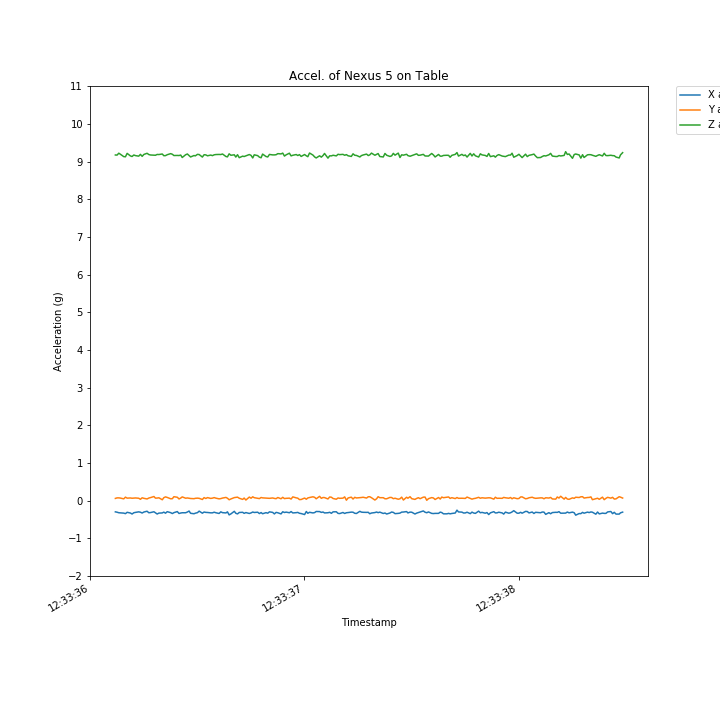
\includegraphics[scale=0.25]{won_table}
%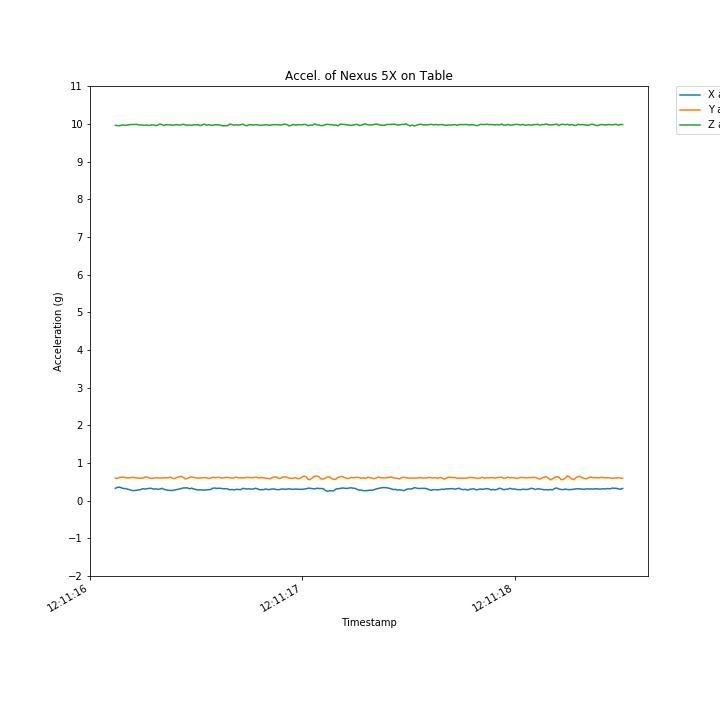
\includegraphics[scale=0.25]{joanna_table}
%\caption{Graphs of the acceleration of the Nexus 5 and 5X while on a table (at different times).}
%\end{figure}

Our goal is to allow the classifier to predict phone states no matter what action the user may be performing.
This includes times when the phone is not physically on the user, including cases that may be very difficult to differentiate: a phone being in a still backpack versus on a table, for example.
Later, we propose a potential solution to this problem. 


\subsection{Features}
For creating features, the relevant sensor data were the accelerometer readings (X, Y, Z values), number of unlocks, number of screen touches, and number of times the screen turned on/off. 
For each window of 0.5s of these raw sensor readings, we generate the following features:

\begin{enumerate}
\item \textit{Total number of phone unlocks}
\item \textit{Total number of phone touches}
\item \textit{Fraction of window that phone screen was on}
\item \textit{Mean acceleration in each of X, Y, Z}
\item \textit{Std. deviation of acceleration in each of X, Y, Z}
\item \textit{Mean magnitude of acceleration in each of X, Y, Z}
\item \textit{Std. deviation of magnitude of acceleration in each of X, Y, Z}
\item \textit{If phone is flat (handcrafted feature explained below)}
\end{enumerate}

The ``If phone is flat" feature was a boolean feature derived from the raw accelerometer readings. 
The feature was 1 if equations 1,2,3 below held true, and 0 otherwise.

\begin{equation}\label{eq1}
 \text{(Mean X Accel. Magnitude)} < 1.0 
\end{equation}

\begin{equation}\label{eq2}
\text{(Mean Y Accel. Magnitude)} < 1.0
\end{equation}

\begin{equation}\label{eq1}
\hspace*{-1cm}|9.8 - \text{(Mean Z Accel. Magnitude)}| < 1.0
\end{equation}

Other sensors that we considered to be relevant with predicting phone states are batched light and step count.
However, the batched light sensor was not used because of its inability to distinguish outdoor nighttime darkness and the darkness from an enclosed backpack. 
We could not use the step count sensor because the sensor data we collected showed that this sensor was not reliable. 

We do not utilize a overlapping or `rolling` window, and instead take distinct chunks of 0.5 seconds.
We believe that this is acceptable since the window size is small enough that we would not miss most transitions.
This decision is supported by previous work that showed there is no notable difference in accuracy between using overlapping and non-overlapping windows \cite{Martin2013}

\subsection{Architecture}
Our architecture has two parts.
The first consists of convolutional layers, while the second part contains dense fully connected layers.


\begin{figure*}[!h]
  \vspace{-0.2cm}
  \centering
   {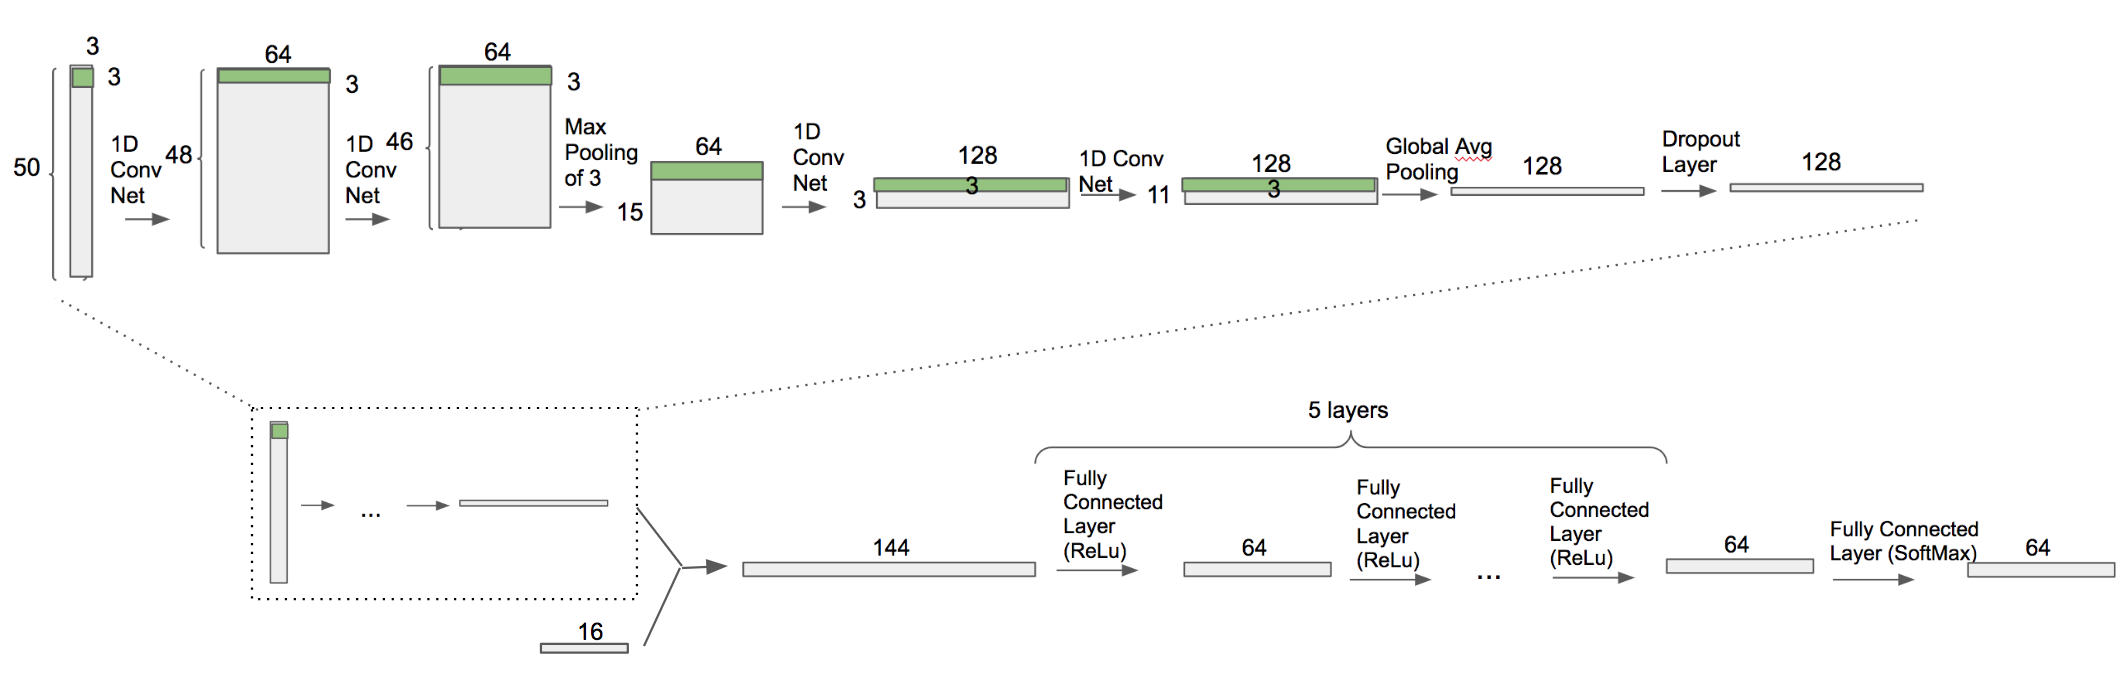
\epsfig{file = convnet1, width = \linewidth}}
  \caption{The architecture of our convolutional neural net}
  \label{fig:ConvNet}
  \vspace{-0.1cm}
\end{figure*}


\begin{table}[!h]
\begin{center}
\begin{tabular}{llrp{2.5cm}}\toprule
Layer 	&  	 	Filters 	& 	Outputs  	&  	Activation \newline / Note\\\midrule
Conv1D  	&  	64 		& 	$48 \times 3$	&  ReLU \\
Conv1D  & 	64 		&	$46 \times 3 $ 	& ReLU  \\
MaxPooling1D  &  64 		& 	$15 \times 3$	& Stride = 3\\
Conv1D & 		128 	& 	$13 \times 3$&  ReLU\\
Conv1D & 128 & $11 \times 3$ & ReLU\\
GAP1D & 128 & $128 \times 1$ & \\
Dropout & | &  $128 \times 1$ & Rate = 0.5\\
Concat  & | & $144 \times 1$&  ($128 \times 1$) \newline + ($16 \times 1$)\\
Dense & | & 64 & ReLU; 6 of these in succession \\
Dense & | & 4 & Softmax

\end{tabular}
\caption{Model Architecture. For all convolutional layers, the kernel was $3 \times 6$, and GAP1D is short for GlobalAveragePooling1D. In the concatenation layer, the count features ($16 \times 1$) are concatenated with convolutional outputs to form the initial input into the dense layers.}
\label{tab:ArchDescription}
\end{center}
\end{table}

In the convolution section, we use the raw acceleration data, which includes the acceleration in the x, y, z directions. 
After multiple one-dimensional convolution layers, max and global pooling, and dropout layers, 
we concatenate the 16 features above in order to incorporate the features that do not involve the data from the accelerometer.  
Together, these features are fed into the second part of the net.  
We chose to separate the features in this way in order to take advantage of the potentially periodic behavior of a user's acceleration in certain positions (e.g. walking).
The features that use the acceleration in the X, Y, Z are separated from the other binary features because we wanted to capture the time series data of the different phone states.
The other binary features are independent of the time, so these features are added in after the acceleration features go through the convolution layers.  

After the concatenation of inputs, our model has 6 dense layers culminating in 4 outputs, which match the four classes listed previously. 
Our model is shown in Figure ~\ref{fig:ConvNet} and a description is shown in Table ~\ref{tab:ArchDescription}.
We have experimented with other architecture, such as separate binary linear classifiers for each phone state and separate neural net classifiers for each phone state.
However, we found out this multiclass neural net classifier works best and has the highest accuracy rates. 
We also experimented with the number of convolutional and dense layers as well as the number of layer units and width of the convolutional filters.

\section{Evaluation}

\subsection{Data Collection Tools}
\subsubsection{Data Collection Software}
The software used to collect data for this experiment is the AppMon logging mobile application 
for the Android phone. 
The AppMon application logs the smartphone sensors, including the following:
\begin{enumerate}
\item Accelerometer
\item Number of unlocks
\item Number of screen touches
\item Number of times the screen turns on and off
\end{enumerate}

In our project, we will be using data from the sensors
to create features in order to classify and predict the location of the phone. 

The app collects accelerometer readings (X, Y, Z directions) in units of $m/s^2$ every 10ms.
It also registers the timestamp at which various trigger events occur (e.g. phone unlocks, screen on, etc.)

\subsubsection{Phones}
We used two phones for the purpose of diary studies and collecting data for creating the classifiers.
One phone was a Nexus 5 and the other was a Neuxs 5s


\subsection {Diary Study}
To obtain data for training and validation, one participant used the test phone with the app installed 
and underwent a daily routine.
Whenever a change of state occured [Note: As of this point, would the reader know what the states are?], the participant would record the time (according to the phone) and the new state.


The distribution of the states during the diary study are shown below:


\begin{center}
\begin{tabular}{ |c|c| } 
 \hline
 Table & To \\ 
 Backpack & DO \\ 
 Hand & By \\ 
 Bag & Steven \\ 
 Pocket & Choi \\
 \hline
\end{tabular}
\end{center}
[Enter distribution stuff here @Steven]
\section{Results}
\subsection{Single Phone Model}
Using the architecture detailed in Section 3, we trained the network for 10 epochs
and measured its effectiveness using $10$-fold cross-validation.
Training/validation data was compiled from the diary study conducted with the Nexus 5X.

The average accuracy across all folds was $92.06\%$, and the corresponding
confusion matrix is shown in Figure X. The network is able to learn how to 
classify the Table state very accurately, which is understandable given 
the consistent nature of the state (i.e. always in a still, flat position). The states
of Backpack and Pocket were also classified with pretty moderate accuracy,
with the misclassifications likely stemming from the more diverse nature of 
the two states (i.e. the user could have been moving or still when the phone was
in their backpack or pocket). The Hand state was classified with the least accuracy,
and misclassified most often instead as the Backpack state. These misclassifications
likely also stem from the varied positions of the Hand state, as in addition to the user
using the phone actively in their Hand, they may also walk with their phone inactive
in their hand [@Joanna what kind of hand states did you have?]


\begin{table}[h]
\caption{Confusion matrix of the network predictions. Each entry indicates the proportion of
total instances that were predicted as the predicted class by the network and labeled the actual class.}\label{fig:confusion} \centering
\begin{tabular}{| c || c | c | c | c }  
\toprule
\multicolumn{2}{c}{\textit{Class}}\multicolumn{3}{c}{(Actual)} \\ \cmidrule{1-5}
(Predicted)		&	Backpack    & 	Pocket 	& 	Hand	&	Table \\
\midrule
Backpack			&	0.266 	&	0.005	&	0.024 	&	0.029 \\
Pocket			&	0.016 	&	0.041 	&	0.001 	&	0.001 \\
Hand			&	0.017 	&	0.003 	&	0.035 	&	0.006 \\
Table			&	0.004 	&	0.002 	&	0.002 	&	0.965\\
\bottomrule
\end{tabular}
\end{table}


\subsection{Multiple Phone Models}
We also attempted to validate our networks across different phone models, by training
on data collected by one phone model and then validating on data collected on a 
different phone model. 

However, the same network trained on the Nexus 5X data could unfortunately not be immediately
applied to the Nexus 5 data, as 

We applied this calibration process to both the Nexus 5X and Nexus 5 data, and then
trained a network on all of the Nexus 5X data, and validated individually on each of the 
two days of diary study data collected from the Nexus 5.
Nonetheless, even after calibration, results between the two phones were inconclusive. 
On the first diary study with the Nexus 5 (Diary Study 2), our network
had a validation accuracy of $77.57\%$, significantly lower than the accuracy observed
in the single phone model case. The corresponding confusion matrix shown in figure X.
\begin{table}[h]
\caption{Confusion matrix of the network predictions on Diary Study 2 (Nexus 5).}\label{fig:confusion} \centering
\begin{tabular}{| c || c | c | c | c }  
\toprule
\multicolumn{1}{c}{\textit{Class}}\multicolumn{4}{c}{(Actual)} \\ \cmidrule{1-5}
(Predicted)		&	Backpack    & 	Pocket 	& 	Hand	&	Table \\
\midrule
Backpack			&	0.342 	&	0.016	&	0.017 	&	0.131 \\
Pocket			&	0.001 	&	0.185 	&	0.	 	&	0.000 \\
Hand			&	0.057 	&	0.	 	&	0.004 	&	0. \\
Table			&	0. 		&	0.003 	&	0.	 	&	0.245\\
\bottomrule
\end{tabular}
\end{table}

On the second diary study, with the Nexus 5 (Diary Study 3), our network had a validation
accuracy of $91\%$--an accuracy much more comparable to the cross validation accuracy
demonstrated in the single phone model case. The corresponding confusion matrix is 
shown below in Figure X.

\begin{table}[h]
\caption{Confusion matrix of the network predictions on Diary Study 2 (Nexus 5).}\label{fig:confusion} \centering
\begin{tabular}{| c || c | c | c | c }  
\toprule
\multicolumn{2}{c}{\textit{Class}}\multicolumn{3}{c}{(Actual)} \\ \cmidrule{1-5}
(Predicted)		&	Backpack    & 	Pocket 	& 	Hand	&	Table \\
\midrule
Backpack			&	0.053 	&	0.040	&	0.013 	&	0.001 \\
Pocket			&	0.006 	&	0.037 	&	0.005 	&	0.001 \\
Hand			&	0.	 	&	0.014 	&	0.055 	&	0.001 \\
Table			&	0.009 	&	0.003 	&	0.	 	&	0.763\\
\bottomrule
\end{tabular}
\end{table}


These results suggest that a linear calibration
strategy may be effective, but further investigation is needed for definitive understanding.

\section{Conclusion}
The work described in this paper describes the methodology in applying deep learning to the task of determining the state of a user's smartphone on the user's person. 
To do this, we do not require the user to be performing any specific action.
Instead, we utilize data from the accelerometer and screen, which are both lightweight and readily available on Android phone models, to identify four common phone positions that span most of a user's phone behavior
and appear distinguishable from the sensor data. 
We show that great accuracy can be achieved when evaluating on a single phone model.
Furthermore, we propose an accelerometer calibration strategy for standardizing phone accelerometer
data across phone models, and show the potential generalization of a network trained on data from a single phone model to other phone models. But our cross model results are inconclusive.

\section*{Acknowledgements}
This work could not have been completed without the help and guidance of Serge Egelman, Irwin Reyes, Michael McCoyd, and Jason Xinyu Liu.

This work was supported by NSF through grant CNS-1514457,
by the Hewlett Foundation through the Center for Long-Term Cybersecurity,
by gifts from Qualcomm and Google, and by Intel through the
ISTC for Secure Computing.

\nocite{}

\vfill
\bibliographystyle{ieeetran}
{\small
\bibliography{paper}}


\end{document}
